\chapter{Auswertung der Audiosignale}
\label{Kapitel6}

Das folgende Kapitel richtet sich nun daran die im vorherigen Kapitel aufgenommenen Daten zu verarbeiten und herauszufinden, welche Informationen aus den aufgenommenen Daten abgelesen werden können. Hierzu wird im ersten Schritt eine \ac{FT} auf die einzelnen Datensätze angewandt. Die Ergebnisse der \ac{FT} können dann ausgewertet werden. Es besteht die Vermutung, dass aus den Frequenzspektren der einzelnen Datensätze bereits einige Informationen extrahiert werden können. Inwiefern diese Vermutung korrekt ist und welche sonstigen Erkenntnisse durch die Anwendung der \ac{FT} getroffen werden können wird nun weiter erläutert. 

\section{FT}
Die Theorie hinter der \ac{FT} wurde bereits erläutert, jedoch ist die Umsetzung dieser Theorie innerhalb von Python-Code komplex. An dieser Stelle verzichten wir darauf die genaue Umsetzung der \ac{FT} zu erläutern, da diese bereits durch die Python-Library scipy erfolgt \cite{scipy-fft}. Wie in der Doku erläutert erfolgt die Berechnung der \ac{FT} durch die scipy-Methode \texttt{fft}. Hierbei handelt es sich um eine Implementierung der \ac{FFT}, welche erheblich schneller umgesetzt werden kann. Da es sich bei unserem Signal zusätzlich um ein reelles und homogenes Signal handelt, wie bereits erläutert, kann auch eine RFFT verwendet werden, welche nur den reellen Teil (R) des Signals betrachtet. Durch die Methode \texttt{rfftfreq} lassen sich zusätzlich die Frequenzen berechnen, welche notwendig sind, um das Ergebnis als Frequenzspektrum zu plotten. Um das Ergebnis zu plotten wird die Python-Library matplotlib genutzt. \cite{matplotlib} Mithilfe dieser beider Librarys lassen sich jetzt die Frequenzspektren der einzelnen Signale plotten. 

Die Abbildung \ref{fig:frequenzspektren-fft} zeigt nun exemplarische Frequenzspektren für verschiedene Konfigurationen. Das Keyword ,,Air'' steht hierbei dafür, dass das gezeigte Signal aufgenommen wurde, als der Schleifer in der Luft war, Signalen mit dem Keyword ,,Grinding'' wurden während eines vermeintlichen Schleifprozesses aufgenommen. Die Zuordnung dieser Keywords erfolgt manuell, dadurch kann es Signale mit dem Keyword ,,Grinding'' geben, bei welchem nicht wirklich geschliffen wurde. Genau diese manuelle Zuweisung des Keywords soll durch diese Arbeit automatisiert werden. Zusätzlich enthalten die Abbildungen die Information über die beim Roboter ansteuern festgelegten RPM. Diese festgelegten RPM können als SOLL angesehen werden, das Ziel dieser Arbeit wiederum ist es den IST-Wert der RPM automatisiert zu berechnen. 

\begin{figure}[H]
    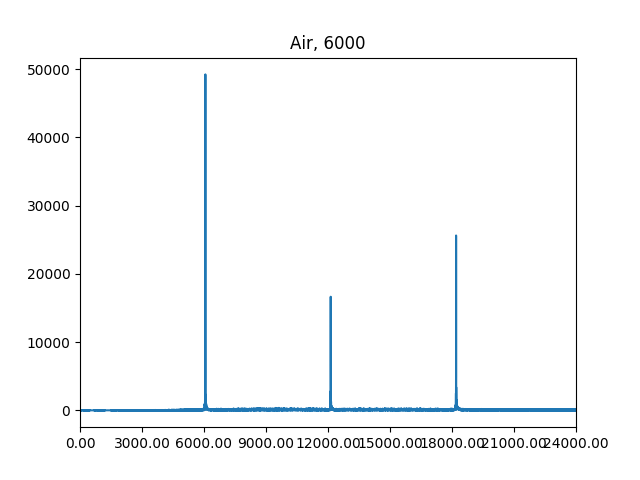
\includegraphics[width=0.5\linewidth]{Studienarbeit//images/Air, 6000, FFT.png}    
    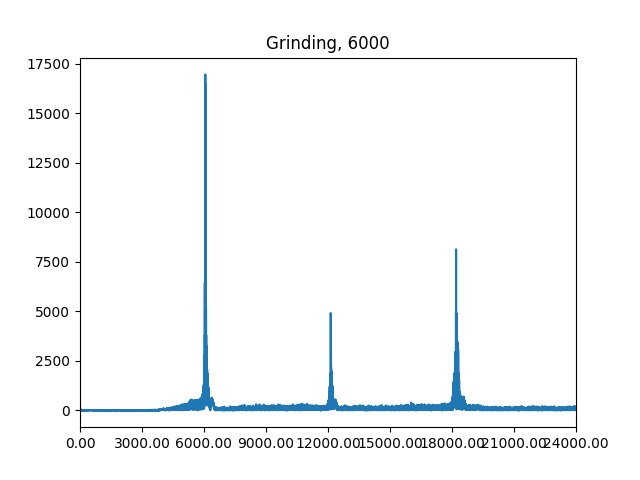
\includegraphics[width=0.5\linewidth]{Studienarbeit//images/Grinding, 6000, FFT.png}
    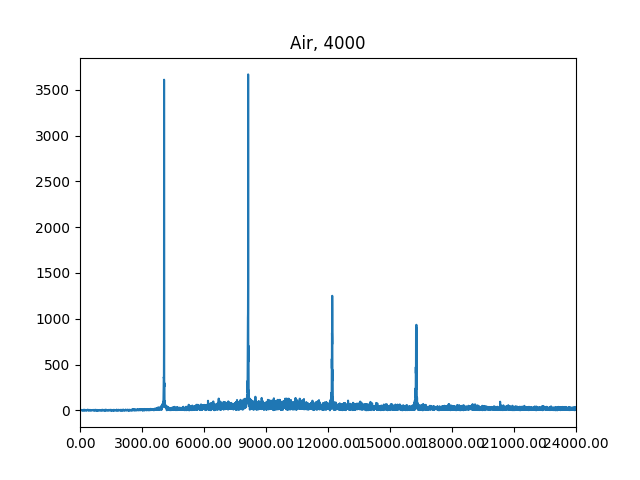
\includegraphics[width=0.5\linewidth]{Studienarbeit//images/Air, 4000, FFT.png}
    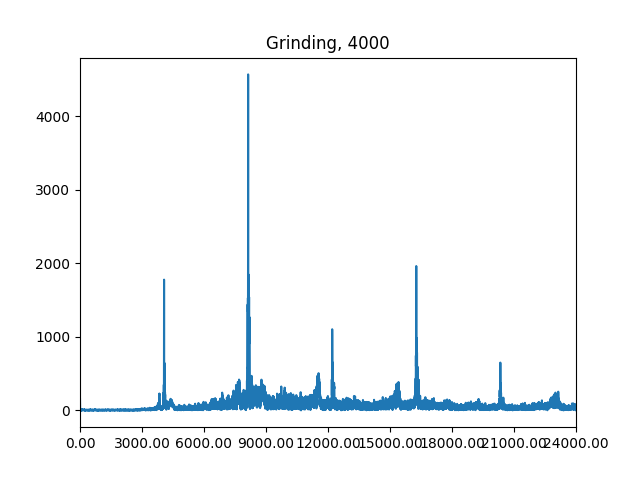
\includegraphics[width=0.5\linewidth]{Studienarbeit//images/Grinding, 4000, FFT.png}
    \caption{Frequenzspektren verschiedener Signale}
    \label{fig:frequenzspektren-fft}
\end{figure}

Die erste Annahme ist, dass der höchste Peak im Frequenzspektrum mit der verwendeten RPM korreliert, da sowohl der Schleifer als auch der Motor Geräusche in diesem Frequenzbereich erzeugen sollten. Wenn man diese Annahme weiterführt, sollten sich bei jedem vielfachen dieser korrelierenden Frequenz ebenfalls ein Peak befinden. Beim betrachten der Abbildungen fällt nun auf, dass dies nicht überall der Fall ist. So ist deutlich zu erkennen, dass diese Annahme bei 6000RPM erfüllt ist, bei 4000RPM ist der höchste Peak jedoch bei 4000 RPM. Stattdessen befindet sich der höchste Peak bei 8000RPM also der doppelten Drehzahl. Woher genau dieser Peak stammt konnte nicht herausgefunden werden, es besteht allerdings die Vermutung, dass durch die 4000 RPM eine Eigenschwingung angeregt wird. Des Weiteren ist es möglich, dass die benutzte Technik hier Probleme aufweist. Um jetzt diese RPM auszulesen bietet es sich an eine Methode zu schreiben, welche alle diese Daten durchgeht und immer dann ein Peak als solchen identifiziert, wenn ein vorher festgelegter Grenzwert überschritten wird. Betrachten wir jedoch die beiden oberen Frequenzspektren fällt auf, dass die Amplitude der Frequenzen sehr unterschiedlich sein kann, so ist es nicht möglich  für jedes Signal den gleichen Grenzwert verwenden kann. Um dies zu beheben müssten nun die Amplituden der Signale normalisiert werden. Diese Normalisierung wird an dieser Stelle zunächst nicht durchgeführt, da durch die bereits aufgeführten Grundlagen die Vermutung auftritt, dass dieses Problem sich durch die Verwendung einer \ac{STFT} oder einer \ac{CWT} lösen lässt. Als Ergebnis lässt sich hier an dieser Stelle bereits festhalten, dass sie die RPM des 6000 gut herauslesen lassen und mit mehr Aufwand bereits dies bereits bei der \ac{FFT} möglich wäre. Das einfache Ablesen durch eine Methode bei 4000RPM ist dies jedoch nicht möglich, da der höchste Wert nicht die RPM widerspiegelt.

Die zweite Eigenschaft, die durch diese Arbeit automatisiert heraus gelesen werden sollte ist die Erkennung, ob der Schleifer tatsächlich geschliffen hat oder die Schleifleistung nicht wie erwartet erfolgt ist. Betrachten wir uns wieder die Abbildung \ref{fig:frequenzspektren-fft} sehen wir, dass die Frequenzspektren der Signale mit der Angabe ,,Grinding'' viel mehr kleinere Spikes besitzen. Auch hier fällt wieder auf, dass bei 4000RPM auch in der Luft das Frequenzspektren viele kleine Spikes aufweist, dies verstärkt wiederum die Vermutung, dass irgendwas die Frequenzen dort verstärkt und verrauscht. Um nun automatisiert zu ermitteln, ob in dem vorhandenen Datensatz geschliffen wurde, könnte man auch hier eine Methode implementieren, welche die Anzahl der Peaks zählt und einen Grenzwert festlegen, ab welchem ein vorliegendes Signal mit dem Zusatz ,,Grinding'' klassifiziert wird. Eine Alternative dazu ist die Ermittlung des Signal-Rausch-Verhältnis des Frequenzspektrum, wenn nun das SNR berechnet wurde, kann auch hier ein Grenzwert festgelegt werden. Bei diesen beiden Grenzwerten tritt ähnlich wie bei der Festlegung des Grenzwertes für die RPM Bestimmung das Problem auf, dass sich der Grenzwert hier für jedes Signal Unterscheiden kann. An dieser Stelle stellt sich auch die Vermutung auf, dass dieses Problem durch die Nutzung einer \ac{STFT} oder \ac{CWT} gelöst werden kann, da durch die \ac{STFT} und die \ac{CWT} das Signal besser normalisiert wird.

Zusammenfassend lässt sich an dieser Stelle sagen, dass es den Anschein erweckt, dass aus den vorliegenden Daten Informationen über die RPM und die Schleifleistung extrahiert werden können. Diese Daten könnten vielleicht durch die Entwicklung komplexer Algorithmen für die Grenzwertfestlegung der Amplitude, der Peakanzahl und für das SNR berechnet werden. Die Implementierung dieser Methoden erfolgt an dieser Stelle aber zunächst nicht, da die Vermutung besteht, dass durch die Anwendung einer \ac{STFT} oder \ac{CWT} die gewünschten Informationen schneller und weniger komplex ausgelesen werden können, da bei beiden das Eingangssignal durch die Beibehaltung der zeitlichen Komponente besser normalisiert werden kann. Durch diese Normalisierung, können dann mehr unterschiedliche Signale analysiert werden, wodurch die Fehleranfälligkeit sinken würde. Um diese Vermutung zu überprüfen erfolgen nun in den nächsten Unterkapiteln die Durchführung einer \ac{STFT} und einer \ac{CWT}, mit dem Ziel Informationen über die RPM und die Schleifleistung mit einer höheren Zuverlässigkeit bereitstellen zu können.


\section{STFT}
Dieses Kapitel richtet sich nun daran die Audiosignale mithilfe einer \ac{STFT} zu analysieren. Die Grundlagen, wie eine solche \ac{STFT} funktioniert wurde schon bereits erläutert. Die Phyton Implementierung der \ac{STFT} findet durch die bereits für die \ac{FT} verwendete Phyton-Library scipy statt. Diese Implementierung basiert auf dem vorgestellen Algorithmus von Cooley und Tukey \cite{scipy-stft}. Um nun \ac{STFT} mit dieser Bibilothek durchführen zu können muss zunächst das Fenster festgelegt werden, welches danach Schritt für Schritt über das Signal gelegt werden kann. Zusätzlich muss der Versatz festgelegt werden. Um trotz der Überlappung möglichst viele Informationen extrahieren zu können bietet es sich an ein nicht lineares Fenster zu benutzen. Ein weit verbreitetes Fenster ist das Gaussian-Fenster, welches Glockenförmig ist und somit Daten in der Mitte des Fensters eine höhere Gewichtung gibt. Diese höhere Gewichtung ist sinnvoll, da die Daten am Rand des Fensters durch die Überlappung doppelt ausgewertet werden. Zusätzlich lässt sich bei diesem Gaussian-Fenster die Standardabweichung festlegen, welche die Glocken-breite bestimmt. Die Form und Länge des Fensters bestimmt das Ergebnis der \ac{STFT}, um herauszufinden, welche Parameter für den spezifischen Anwendungsfall am besten geeignet sind, müssen verschiedene Parameter verglichen werden.

\paragraph{Parameterwahl}
Die Abbildung \ref{fig:parameter-stft} zeigt die Anwendung verschiedener Versätze (\(\Delta t\)) und Fenster-Längen und Standardabweichungen des Gaussian-Fenster (\(\sigma\)) zu erkennen. Hierbei wurde als Signal mit 6000RPM und der Klassifizierung ,,Air'' gewählt und der Länge von 60s gewählt.

\begin{figure}[H]
    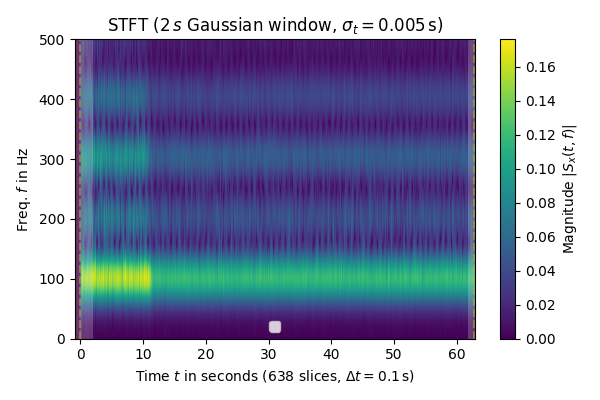
\includegraphics[width=0.5\linewidth]{Studienarbeit//images/2sr-1_400-sr_10.png}    
    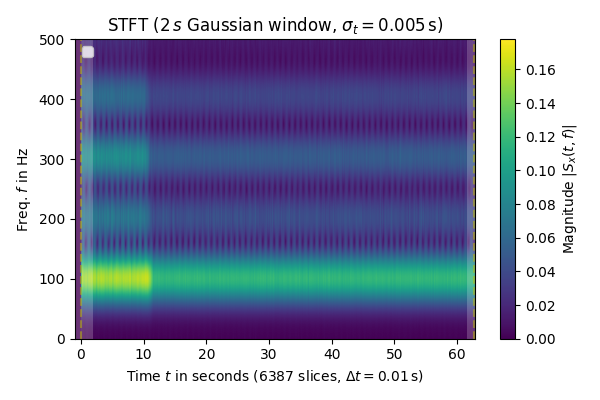
\includegraphics[width=0.5\linewidth]{Studienarbeit//images/2sr-1_400-sr_100.png}
    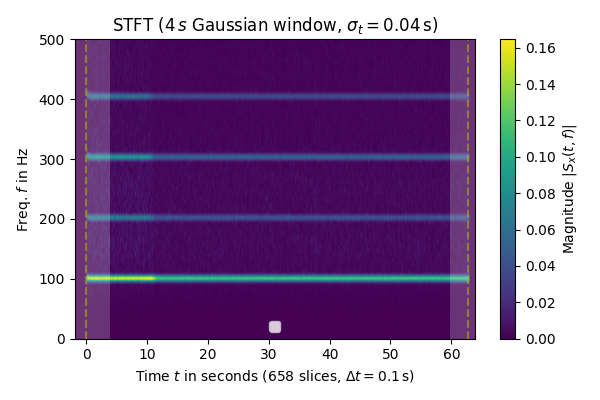
\includegraphics[width=0.5\linewidth]{Studienarbeit//images/4sr-1_100-sr_10.png}
    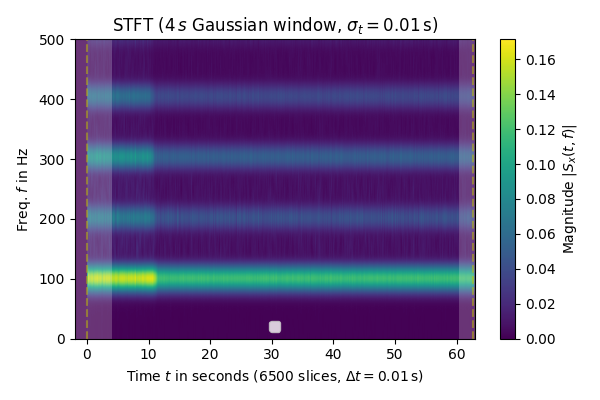
\includegraphics[width=0.5\linewidth]{Studienarbeit//images/4sr-1_400-sr_100.png}
    \caption{Auswirkung verschiedener Parameter auf die STFT}
    \label{fig:parameter-stft}
\end{figure}

Wie bereits im Grundlagen Kapitel \ref{Kapitel2} erläutert muss man sich je nach Anwendungsfall für Zeit- oder Frequenzgenauigkeit entscheiden, da bereits durch die \ac{FFT} auffällt, dass die Schleifgeräusche nicht besonders deutlich zu erkennen sind, scheint hier eine Fokussierung auf die Frequenzgenauigkeit sinnvoll, um die wenigen Informationen die man hat möglichst detailiert auszuwerten. Wie in der Abbildung \ref{fig:parameter-stft} erkennbar erreicht man eine diese durch die Verlängerung des Fensters. So sind die Frequenzen viel detaillierter in den beiden unteren Abbildungen mit einer Fenstergröße von 4s zu erkennen, als bei 2s. Eine noch höhere Genauigkeit wird durch die Vergrößerung der Standardabweichung \(\sigma\) erreicht, zu erkennen in den unteren Bildern. Zusätzlich erhöht sich jedoch die Zeitliche Genauigkeit durch Verringerung des Versatzes (\(\Delta t\) auf der X-Achse). Da besonders der Fokus auf die Frequenzen notwendig ist, wird sich an dieser Stelle für eine Fenstergröße von 4s entschieden, dies der 4-fachen sampling-rate entspricht. Zusätzlich wird ein Versatz von 0,1s, also 1/10 der sampling-rate als sinnvoll betrachtet. Für die Standardabweichung wird sich für 0,04s entschieden, dies entspricht 1/100 der Fensterbreite. Diese Wahl der Parameter sorgt dafür, dass die Frequenz und deren Schwankungen sehr genau abgebildet werden und trotzdem noch genügend Informationen vorhanden sind, um zeitliche Angaben zu treffen.

\paragraph{Auswertung verschiedener Datensätze}
Da nun die Wahl der Parameter erfolgt ist, werden nun verschiedene Datensätze mithilfe einer \ac{STFT} und diesen gewählten Parametern ausgewertet. Die Abbildung \ref{fig:verschiedene-stft} zeigt mehrere repräsentative Ergebnisse. Die Beschriftungen der Abbildungen ist wie auch bei der \ac{FFT} gewählt.

\begin{figure}[H]
    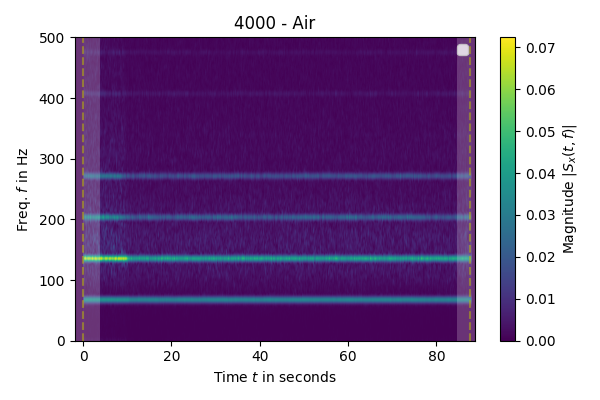
\includegraphics[width=0.5\linewidth]{Studienarbeit//images/stft-4000-air.png}    
    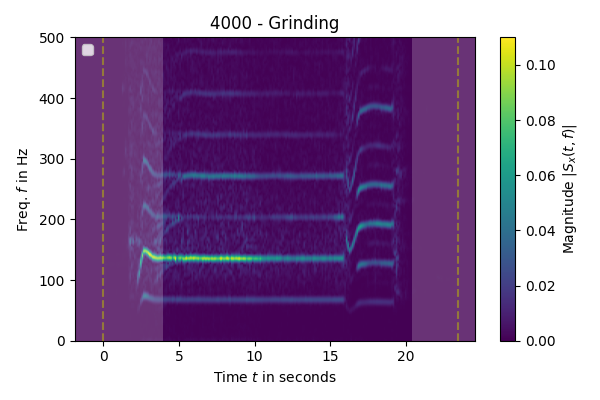
\includegraphics[width=0.5\linewidth]{Studienarbeit//images/stft-4000-grinding.png}
    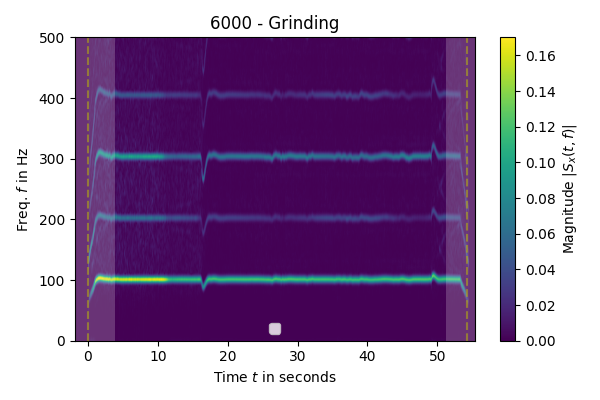
\includegraphics[width=0.5\linewidth]{Studienarbeit//images/stft-6000-grinding.png}
    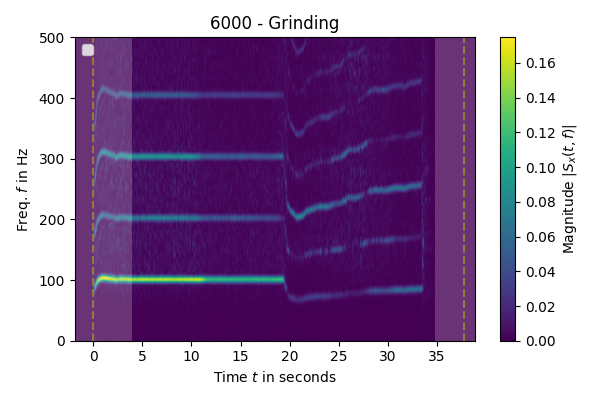
\includegraphics[width=0.5\linewidth]{Studienarbeit//images/stft-6000-grinding-hard.png}
    \caption{Anwendung der STFT auf verschiedene Signale}
    \label{fig:verschiedene-stft}
\end{figure}

Ähnlich wie auch bei der \ac{FFT} ist in den Abbildungen deutlich zu erkennen, dass eine Frequenz stärker heraus sticht, als die anderen. Bei einem SOLL von 4000 RPM sticht die Frequenz von \textasciitilde 130Hz besonders hervor, 130HZ entsprechen hier \textasciitilde 8000RPM. Das verstärkte Auftreten der doppelten Frequenz bei SOLL-4000RPM wurde bereits bei der \ac{FFT} beobachtet. Die Gründe dafür bleiben weiter unbekannt. Da diese Verstärkung jedoch immer auftritt und auch über die gesamte Audiolänge hinweg, kann davon ausgegangen werden, dass dies vom Motor des Schleifers selbst stammt. Bei den SOLL von 6000RPM liegt die gemessene Frequenz bei \textasciitilde 100HZ, was wiederum 6000RPM entspricht. Da dieser Peak konstant zu sein scheint, lässt sich daraus die IST-RPM berechnen, mehr dazu im nächsten Abschnitt. Vorher betrachten wir die beiden rechten Abbildungen. Bei beiden ist am Ende eine Verwischung der Frequenzen zu erkennen. Interessant hierbei ist, dass beim Aufnehmen dieser beiden Audiospuren der Schleifer am Ende zu stark auf das Material gedrückt hat. So stellt sich hier die Vermutung auf, dass es sich bei der zu sehenden Anomalie um einen zu hohen Anpressdruck handelt. Diese Vermutung wird an späterer Stelle nochmals aufgegriffen. Eine weitere zu erkennende Anomalie ist, dass in jedem Audiosignal in den ersten 10 Sekunden die Frequenzen stärker ausgeprägt scheinen. Ein Grund dafür lässt sich auch nur vermuten, aber da die Frequenz hierbei konstant bleibt und der Zeitraum der Verstärkung immer am Anfang der Aufnahme liegt, liegt die Vermutung nahe, dass es sich möglicherweise um Resonanzen im Aufnahmesystem oder elekrisches Rauschen handelt. Da dieses Rauschen in jedem Audiosignal gleich stark aufzutreten scheint, kann dies vernachlässigt werden.

Um nun die RPMs berechnen zu können wird eine Methode implementiert, welche die maximale Ausprägung einer Frequenz findet. Da durch die \ac{STFT} auch eine zeitliche Komponente enthalten ist, liegt die Entscheidung nahe die RPMS nicht für die gesamte Audiospur, sondern immer für kleine Teile zu berechnen. Im Sinne der reellen Anwendung scheint hierbei eine Auswertung auf Sekunden-ebene sinnvoll. Nachdem die am stärksten ausgeprägte Frequenz gefunden wurde lässt sich diese mit 60 multiplizieren um RPMs zu erhalten. Der Algorithmus geht also Sekunden-weise durch die Ergebnisse der \ac{STFT} durch und sucht immer die am stärksten ausgeprägte Frequenz. Die Abbildung \ref{fig:rpm-stft} zeigen nun die berechneten RPMs für die in der Abbildung \ref{fig:verschiedene-stft} gezeigten Datensätze, zusätzlich ist auf den Diagrammen die Stärke der Ausprägung (Intensity) angegeben, zur Veranschaulichung ist diese Ausprägung mit einem Faktor von 100000 multipliziert.

\begin{figure}[H]
    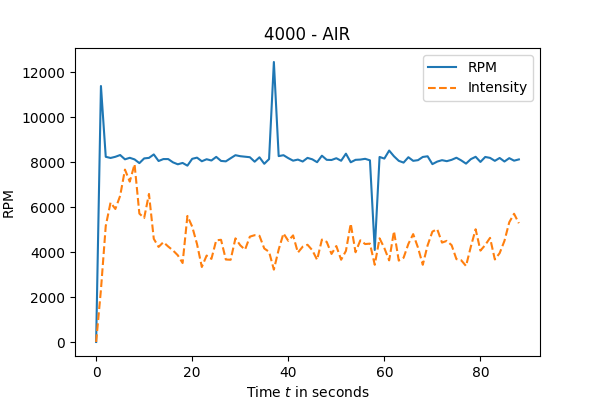
\includegraphics[width=0.5\linewidth]{Studienarbeit//images/stft-rpm-4000-air.png}    
    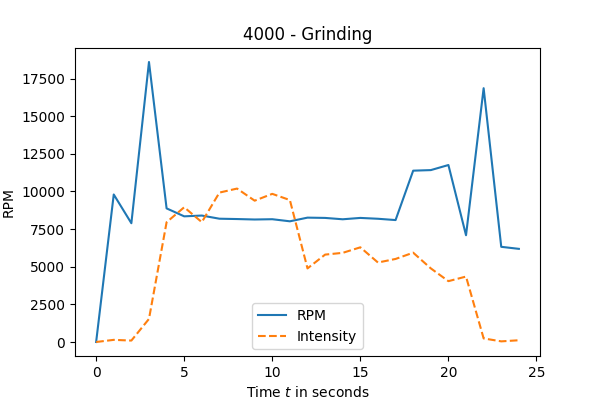
\includegraphics[width=0.5\linewidth]{Studienarbeit//images/stft-rpm-4000-grinding.png}
    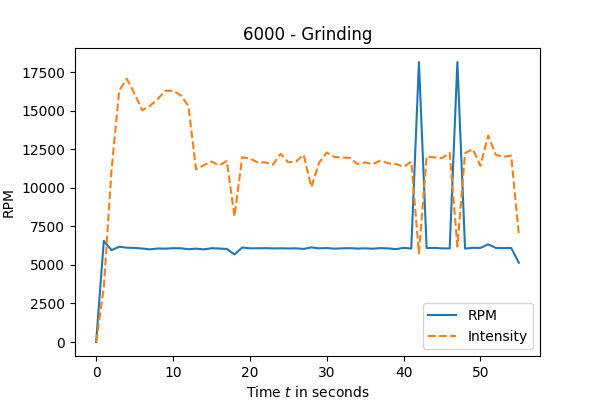
\includegraphics[width=0.5\linewidth]{Studienarbeit//images/stft-rpm-6000-grinding.png}
    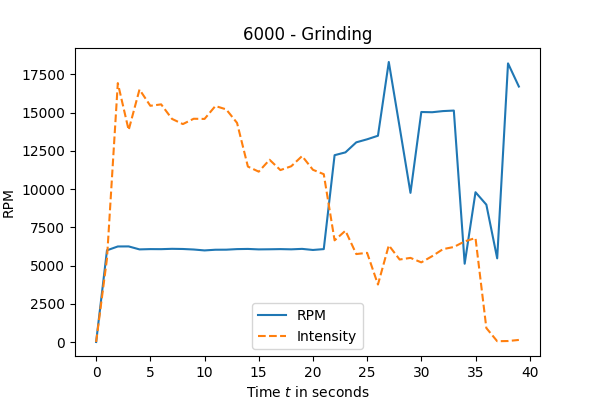
\includegraphics[width=0.5\linewidth]{Studienarbeit//images/stft-rpm-6000-grinding-hard.png}
    \caption{Berechnung der RPM durch die STFT}
    \label{fig:rpm-stft}
\end{figure}

Wie bereits erwartet und auch sowohl bei der \ac{FFT} als auch bei der \ac{STFT} sichtbar, weißt die berechnete RPM bei SOLL-4000 eine Abweichung auf und es wird ein IST von 8000 RPM berechnet. Die Quelle für dieses akustische Rauschen in den Audiosignalen im Bereich von 4000 RPM konnte jedoch nicht gefunden werden, es besteht weiterhin die Vermutung, dass es sich hierbei um ein Rauschen handelt, welches durch die Eigenfrequenz des Schleifers ausgelöst wird. Für die Datensätze mit einem SOLL von 6000 RPM erzielt die Methode gute Ergebnisse, jedoch gibt es auch hier Abweichungen. So treten immer dann Abweichungen auf, wenn in der \ac{STFT} Anomalien auftreten, welche vielleicht auf die Schleifleistung zurückzuführen sind, zu sehen in den linken Plots. Interessant ist auch die Intensität der RPM, so ist die Intensität bei den mit ,,Grinding'' markierten Diagrammen immer dann höher, wenn auch die korrekte IST-RPM berechnet wurde. Bei den in der Luft aufgenommenen Datensätzen ist die Intensität auch niedriger. Daraus lässt sich die Vermutung aufstellen, dass die Intensität während der Erbringung einer guten Schleifleistung höher ist. Sinkt die Intensität, so steigt oder sinkt der Anpressdruck so stark, dass die Schleifleistung beeinträchtigt wird. Einen wirklichen Grenzwert lässt sich hierfür jedoch nicht festlegen.

Insgesamt lässt sich an dieser Stelle festhalten, dass es teilweise möglich ist die richtigen RPM zu berechnen, jedoch ist diese Berechnung fehleranfällig. Zusätzlich lassen sich aus den Plots Vermutungen über die Schleifleistung aufstellen. Dennoch haben wir uns entschieden den Ansatz der \ac{STFT} nicht weiter zu Verfolgen. Die \ac{STFT} hat ihren Zweck in der Arbeit erfüllt, in dem Sinne, dass durch die Anwendung aufgezeigt wurde, dass die zeitliche Komponente in diesem Anwendungfall wichtig ist, zusätzlich hat es Beweise dafür geliefert, dass in den Daten Informationen über die RPM und die Schleifleistung enthalten sind. Durch das analysieren vorhandener State-of-the-Art Methoden im Kapitel \ref{Kapitel3} wurde aufgezeigt, dass es eine Methode gibt, welche zwar teilweise komplizierter zu implementieren ist, jedoch im direkten Vergleich wesentlich detailliertere Ergebnisse liefert. Die Rede ist von der \ac{CWT}. Dies ist der Hauptgrund dafür, dass wir uns an dieser Stelle uns dafür entscheiden nicht tiefer die Ergebnisse der \ac{STFT} zu analysieren und stattdessen die grobe Ergebnisse als Machbarkeitsbestätigung zu interpretieren und die genaueren Analysen mithilfe der \ac{CWT} durchzuführen. 


\section{Auswertung mithilfe von CWT}
Wie bereits erwähnt, findet nun die Auswertung mithilfe der \ac{CWT} statt. Hierfür verwenden wir eine auf \cite{Torrence1998} basierende Python-Bibliothek, welche bereits im Kapietel \ref{Kapitel3} ausführlich erläutert wurde. Die wichtigsten Punkte werden hier nun nochmal zusammengefasst.

Um verschiedene Frequenzen isolieren zu können, werden die oben genannten Audiospuren mithilfe einer Wavelet-Transformation analysiert. Dabei verwenden wir das Morlet Wavelet, wobei die Transformation unter der Verwendung einer in \cite{Torrence1998} vorgestellten Methode im Fourier-Raum erfolgt. Wie bereits in Kapitel \ref{Kapitel3} gezeigt, besteht das Morlet-Wavelet aus einer komplexen Exponentialfunktion, die von einer Gauß'schen Funktion moduliert wird \(e^{i\omega_0 t/s}e^{-t^2/(2s^2)}\), wobei \(t\) die Zeit, \(s\) die Skalierung des Wavelets und \(\omega_0\) eine dimensionslose Frequenz ist. Als Erweiterung zu einer einfachen \ac{CWT} nutzt die Bibilothek einen Signifikanz-Test, welcher die Peaks im Wavelet-Powerspektrum betont. Um die Signifikanz zu testen, muss ein Hintergrund-Fourier-Spektrum gewählt werden. Um nicht stationäre Änderungen in der Varianz zu testen, ist es am besten, das globale Wavelet-Spektrum (GWS) zu wählen, das sich aus dem Zeitdurchschnitt des Wavelet-Leistungsspektrums ergibt. Das Wavelet-Leistungsspektrum ist dann um das GWS (Verteilung als Chi-Quadrat mit zwei Freiheitsgraden) verteilt. Zusätzlich wird ein Filter festgelegt, damit einzelne Frequenzbereiche besser isoliert betrachtet werden können. Die Abbildung \ref{fig:cwt-filter} zeigen nun die Anwendung dieses Filters auf das GWS. Gezeigt wird ein Red-Noise-Filter und dessen inverse.

\begin{figure}[H]
    \centering
    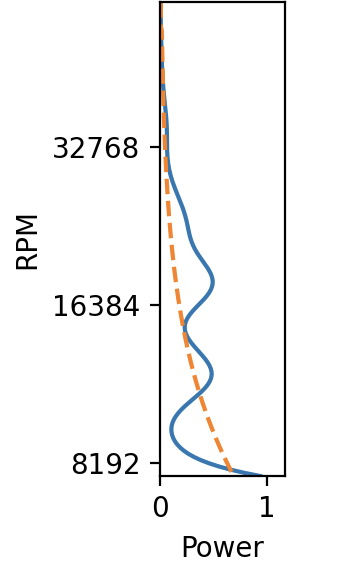
\includegraphics[width=0.25\linewidth]{Studienarbeit//images/cwt-red-noise.png}    
    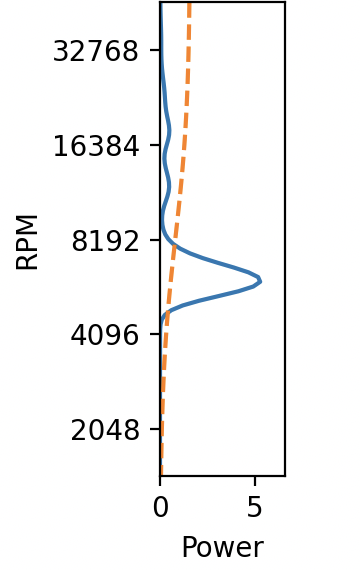
\includegraphics[width=0.25\linewidth]{Studienarbeit//images/cwt-inverse-red-noise.png}
    \caption{Anwendung verschiedener Filter auf das globale Wavelet-Spektrum}
    \label{fig:cwt-filter}
\end{figure}

Zu erkennen ist hierbei, dass durch den Red-Noise-Filter eher die tiefen Frequenzen isoliert werden und durch die inverse die hohen Frequenzen. 

\paragraph{Auswertung der Drehzahl}
Da durch den inversen Red-Noise-Filter vor allem die unteren Frequenzen isoliert werden wird klar, dass dieser Filter sich dazu eignet die Drehzahl zu bestimmen, da diese in diesem unteren Frequenzbereich liegt, wie an dem größten Peaks zu erkennen. Da für die Drehzahl die oberen Frequenzen keine Rolle spielen findet die weitere Verarbeitung mit diesem Filter statt. Wird nun ein Signifikanz-Test mit diesem Filter auf die Ergebnisse der \ac{CWT} angewendet, so entstehen die in der Abbildung \ref{fig:cwt-powerspek-1} gezeigten Plots. Die Beschriftung der Plots erfolgt ähnlich wie auch bei der \ac{STFT} mit der SOLL-RPM und SOLL-Schleifleistung. Die schwarzen Flächen sind jene Flächen, welche durch den Signifikanz-Test heraus gestochen sind, also nicht durch den Red-Noice-Filter ausgefiltert werden.

\begin{figure}[H]
    \centering
    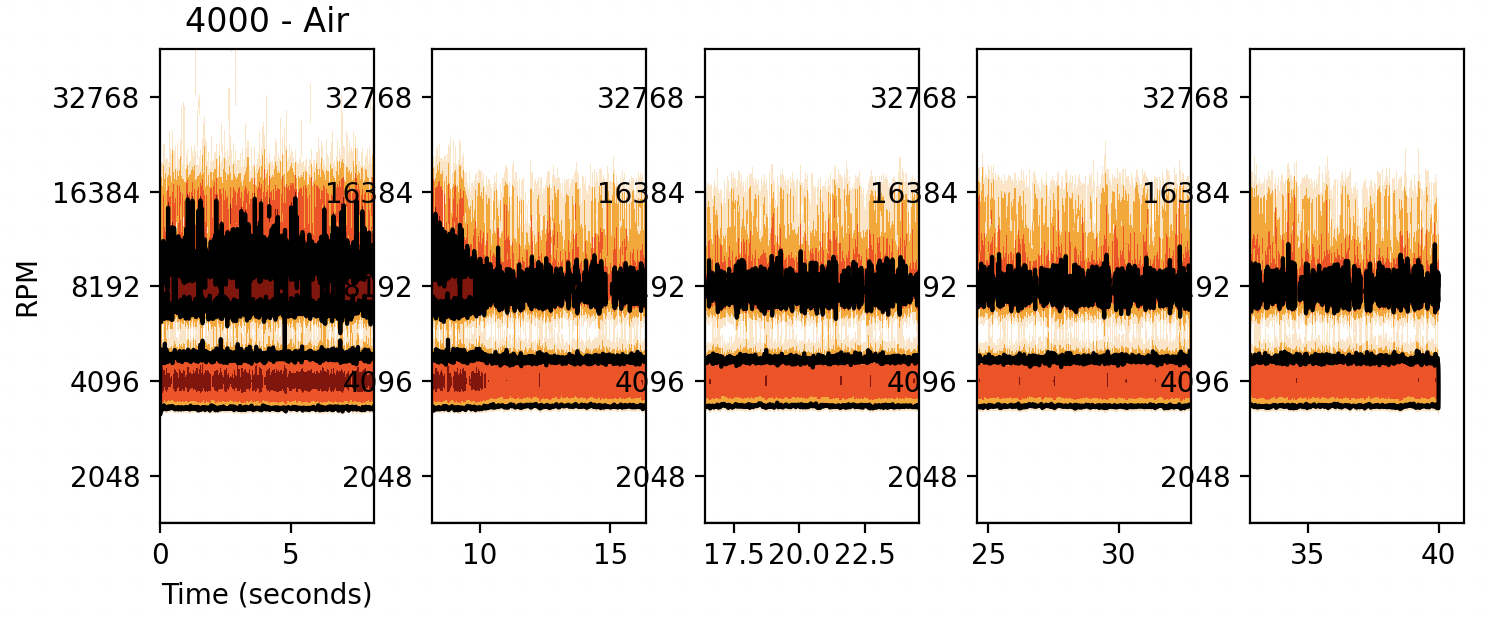
\includegraphics[width=0.8\linewidth]{Studienarbeit//images/cwt-4000-air.png}     
    \centering
    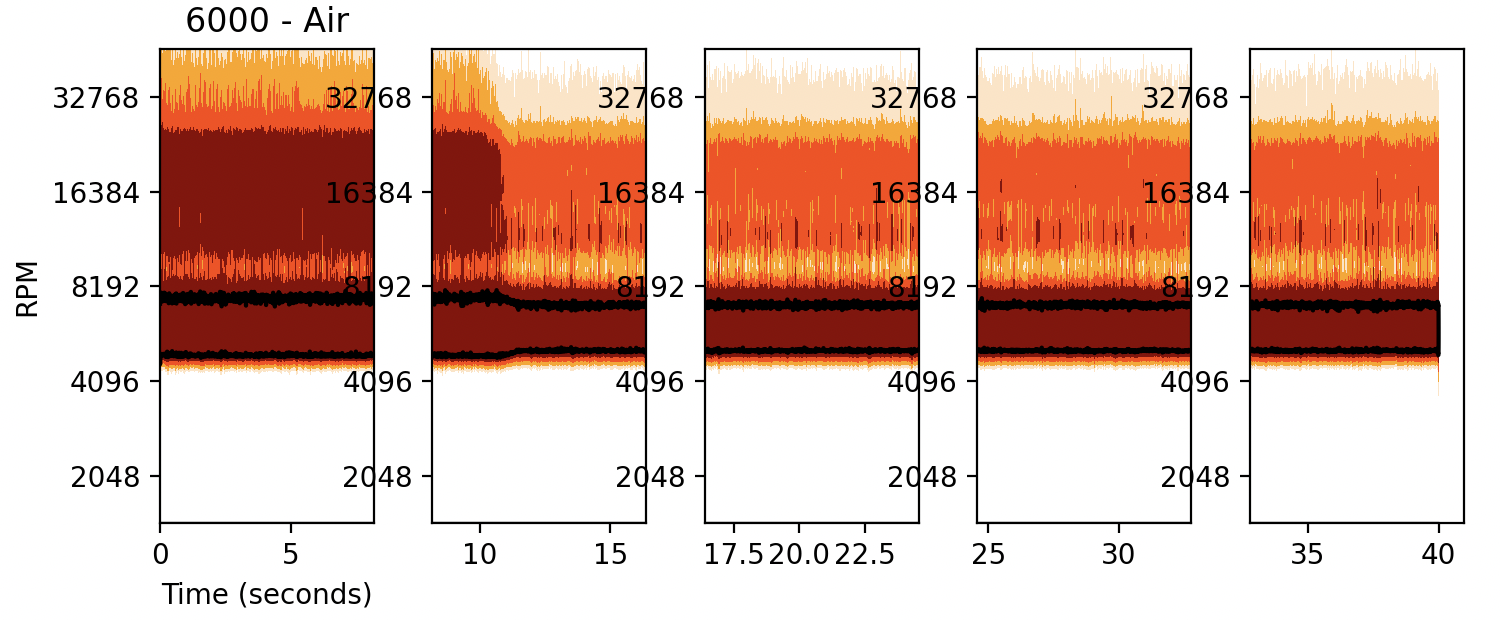
\includegraphics[width=0.8\linewidth]{Studienarbeit//images/cwt-6000-air.png}  
    \centering
    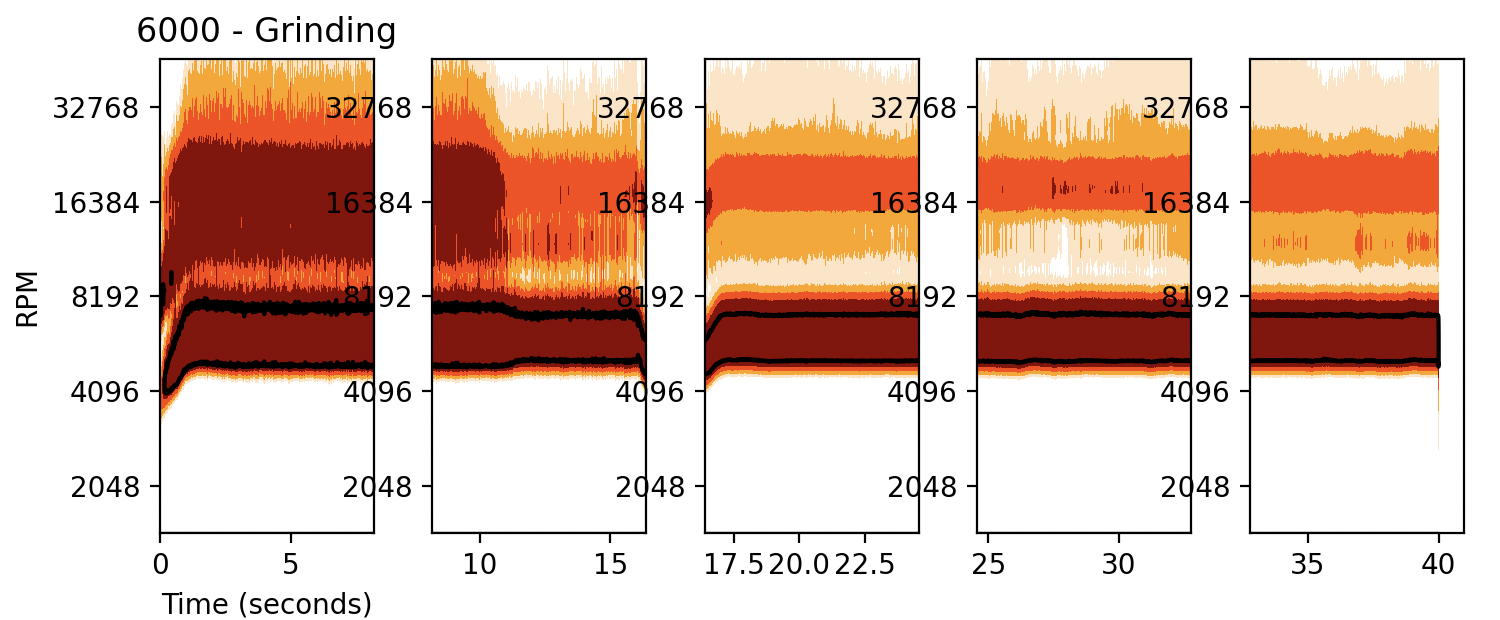
\includegraphics[width=0.8\linewidth]{Studienarbeit//images/cwt-6000-grinding.png}    
    \caption{Powerspektren verschiedener Audiosignale, als Ergebnis der CWT}
    \label{fig:cwt-powerspek-1}
\end{figure}


In der Abbildung deutlich zu erkennen ist, dass die höchsten Frequenzen sich im Bereich von 6000 RPM befinden. Zusätzlich wird deutlich, dass durch den Signifikanz-Test genau diese Frequenz nochmals isoliert wird und somit nur der Bereich um 6000 RPM eine hohe Signifikanz besitzt. Der Signifikante Bereich ist in der gezeigten Abbildung jeweils der, der sich zwischen den schwarzen Linien befinden. Vor allem interessant ist dies, da deutlich wird, dass dieser Bereich sowohl ohne erbrachte Schleifleistung (linkes Bild) als auch mit erbrachter Schleifleistung (rechtes Bild) gleich bleibt. Dies bildet nun den Vorteil gegenüber der \ac{STFT}, bei welcher die Frequenzen bei erbrachter Schleifleistung nicht mehr deutlich sichtbar waren. Durch diese Beobachtung lässt sich nun wiedereinmal eine Methode schreiben, welche immer die Frequenz eines bestimmten Zeitintervalls (z. B. einer Sekunde) ausliest, welche am stärksten ausgeprägt ist und sich gleichzeitig in durch den Signifikanz-Test heraus gestochenen Bereich befinden. So fließt in die Berechnung der höchsten Frequenz nicht nur die lokal stärkste Frequenz ein, sondern auch der globale Durchschnitt. Wendet man diese Methode nun an erhält man die in der Abbildung \ref{fig:cwt-rpm} gezeigten Plots. Auch hier wird nun wieder eine Intensität mit angegeben. Diese Intensität ist die aus der\ac{CWT} stammenden Intensität aber jedoch mit 1000 multipliziert, um die Visualisierung zu Verbessern. 

\begin{figure}[H]
    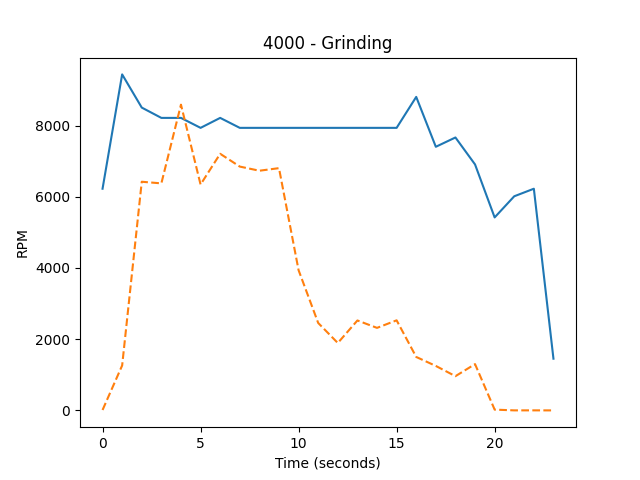
\includegraphics[width=0.5\linewidth]{Studienarbeit//images/cwt-rpm-4000-grinding.png} 
    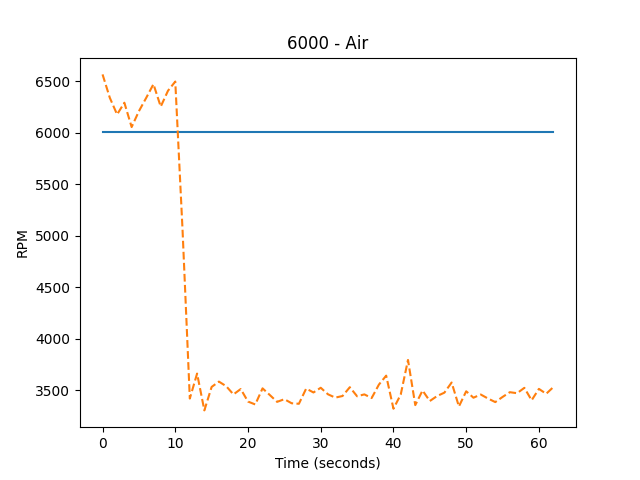
\includegraphics[width=0.5\linewidth]{Studienarbeit//images/cwt-rpm-6000-air.png}    
    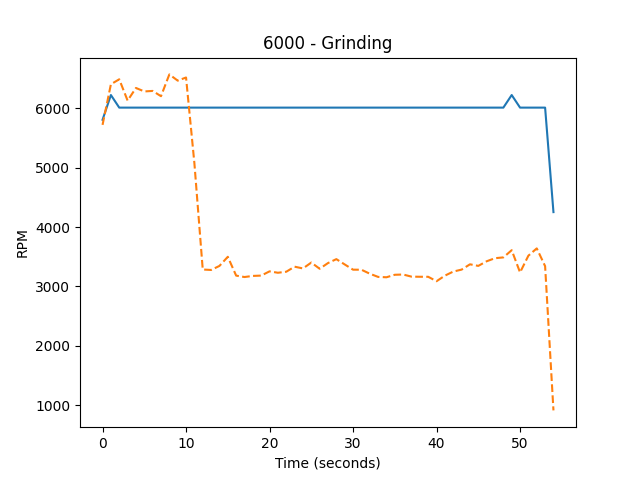
\includegraphics[width=0.5\linewidth]{Studienarbeit//images/cwt-rpm-6000-grinding.png}    
    \caption{Berechnung der Drehzahl auf Grundlage einer CWT}
    \label{fig:cwt-rpm}
\end{figure}


Betrachtet man sich nun diese Ergebnisse, fällt auf, dass die berechneten RPM bei 6000 RPM sehr genau sind und im Gegensatz zu der \ac{STFT} die Berechnung auch dann noch 6000 RPM ausgibt, wenn eine Schleifleistung erbracht wird, was bei der \ac{STFT} nicht der Fall war. Doch auch hier ist wiederum deutlich zu erkennen, dass bei den SOLL-4000 RPM als IST 8000 RPM ausgegeben werden. Dieses Ergebnis war jedoch zu erwarten, da wie bereits in der Abbildung \ref{fig:cwt-powerspek-1} zu erkennen ist, dass bei 4000RPM vor allem die doppelte Frequenz der Drehzahl über dem Signifikanz-Test liegt. Zwar könnte man hier eine Art Gaussian-Glocke über den Peak bei 8000 RPM legen, jedoch würde dies dann nur bei 4000RPM zu einem Ergebnis führen und bei allen anderen Drehzahlen wird das Ergebnis verschlechtert. Festhalten lässt sich an dieser Stelle, dass die Berechnung der Drehzahl auf Grundlage eines Signifikanz-Test auf einer\ac{CWT} hohe Erfolgschancen aufzeigt.


\paragraph{Auswertung von Schleifleistung}
Im letzten Abschnitt wurde die Methode beschrieben, mit welcher mithilfe der\ac{CWT} die RPM ausgerechnet werden können. Dieser Abschnitt richtet sich nun daran die dafür aufgetretenen Beobachtungen genauer zu betrachten und anhand-dessen einen Algorithmus zu finden, welcher den Schleif-Status innerhalb eines bestimmten Zeitintervalls berechnen kann. Wichtig an dieser Stelle zu erwähnen ist, dass die Beobachtungen nur um den Bereich von 6000 RPM gemacht werden konnten und sich dieser Abschnitt nur daran richtet die Schleifleistung um den Bereich von 6000 RPM bestimmen zu können. Betrachtet man sich nun noch einmal die Abbildung \ref{fig:cwt-powerspek-1}, so fällt auf, bei der dreifachen Frequenz des Schleifers häufig Anomalien auftreten, vor allem wenn das analysierte Audiosignal mit dem Label ,,Grinding'' versehen ist. Aus dieser Beobachtung lässt sich die Vermutung ableiten, dass diese Anomalie immer dann auftritt, wenn der Schleifer tatsächlich am Schleifen ist. Diese Vermutung gilt es nun zu überprüfen, indem diese Anomalie isoliert betrachtet wird. Um dies zu erreichen wird der Red-Noise-Filter verwendet, welcher die tieferen Frequenzen herausfiltert. Zusätzlich wird das Morlet-Wavelet so angepasst, dass nur die Frequenzen über 8000 RPM in der\ac{CWT} betrachtet werden. Die Auswahl des Filters und die Regelung dessen Stärke gelingt durch ausprobieren. Inwiefern der Filter angepasst werden muss, wurde durch die Anwendung des Filters auf das GWS verdeutlicht. Wird nun diese angepasste\ac{CWT} und der angepasst Filter des Signifikanz-Test angewendet, so erhält man die in der Abbildung \ref{fig:cwt-powerspek-2} gezeigten Power-Spektren. Rechts neben dem Power-Spektrum ist jeweils das GWS und der Filter zu sehen.

\begin{figure}[H]
    \centering
    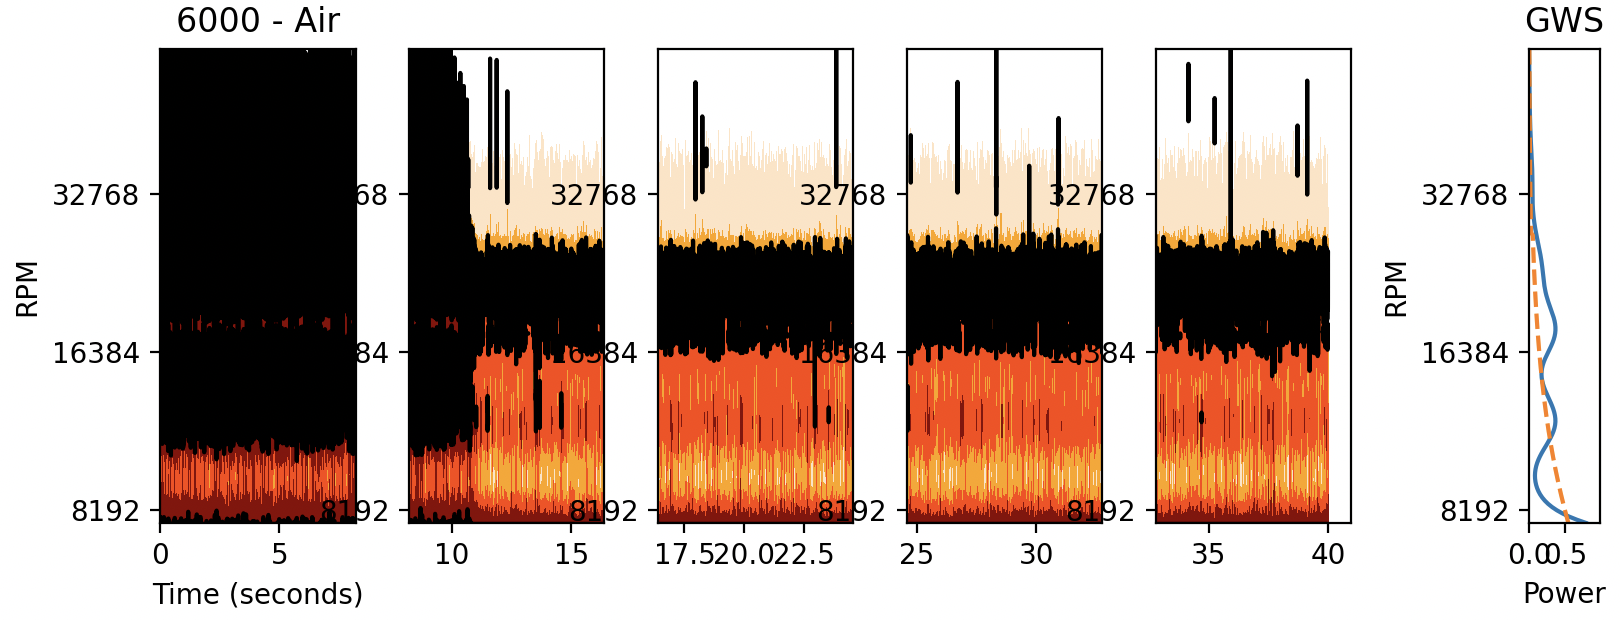
\includegraphics[width=0.8\linewidth]{Studienarbeit//images/cwt-iso-6000-air.png}    
    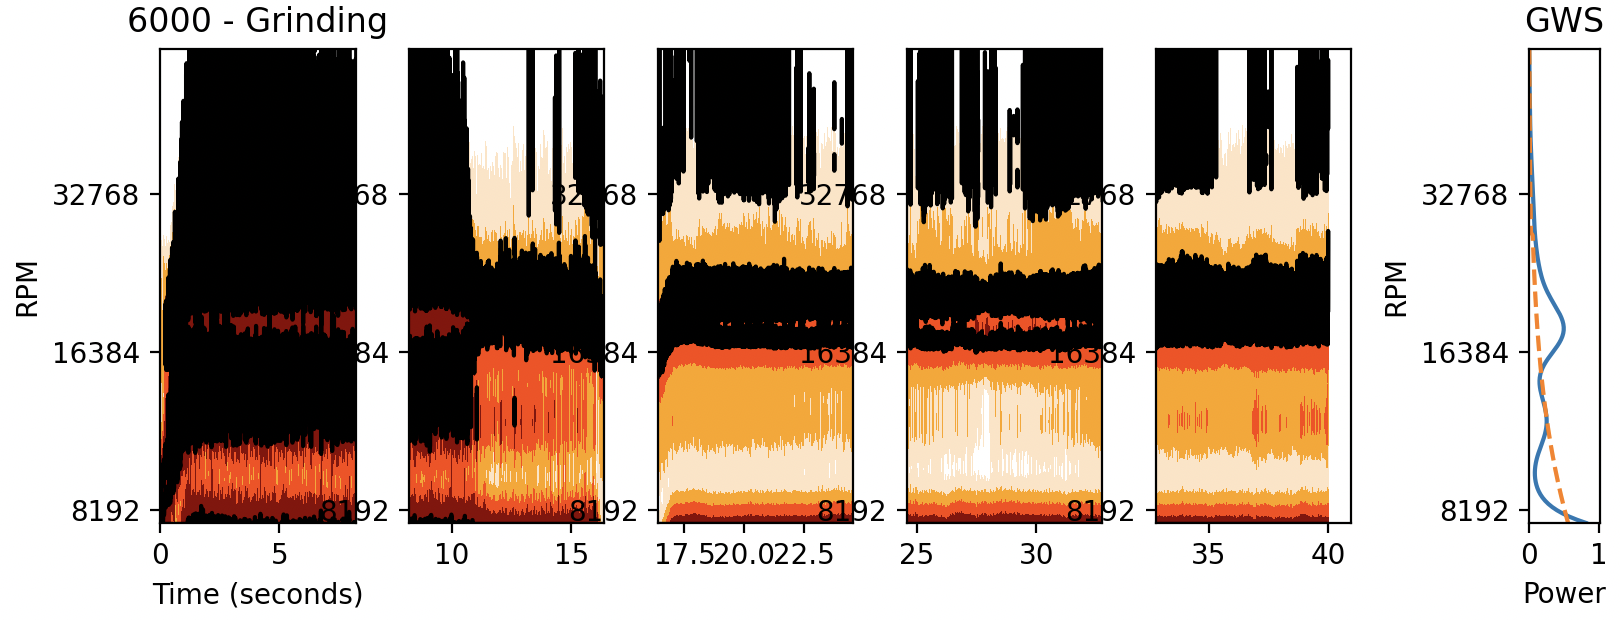
\includegraphics[width=0.8\linewidth]{Studienarbeit//images/cwt-iso-6000-grinding.png}   
    \caption{Powerspektrum isolierter Frequenzen, als Ergebnis der CWT}
    \label{fig:cwt-powerspek-2}
\end{figure}


Wie bereits im vorherigen Kapitel beschrieben markieren die schwarzen Flächen jeweils die Frequenzen, welche durch den Signifikanz-Test aufgefallen sind. Deutlich zu erkennen ist hier, dass der Signifikanz-Test in zwei Bereichen besonders ausschlägt. Bereich 1 ist der bereits vermutete Bereich bei der dreifachen Drehzahl des Schleifer und bei dem mit ,,Grinding'' markierten Datensätze schlägt der Signifikanz-Test auch ab dem Bereich von 32 000 vermehrt an.  Die Ausschläge über 32000 RPM entstehen vermutlich durch Rauschen, welches beim Schleifen des Werkstücks auftreten. Die Quelle dieses Rauschen ist leider unbekannt, womöglich stammt dies vom Material des Werkstücks oder der Schwingung des Werkstücks während des Schleifprozesses. Im nächsten Schritt werden nun diese auftretenden Bereiche genauer analysiert, um herauszufinden, welche Frequenz jeweils besonders heraus-sticht. Um nun die Daten Ergebnisse der\ac{CWT} genauer zu betrachten wird hier nun ähnlich wie auch zu Bestimmung der RPM eine Methode implementiert, welche immer jeweils immer die stärkste Frequenz im Zeitraum einer Sekunde bestimmt. Plottet man nun die Daten erhält man die in der Abbildung \ref{fig:cwt-iso-freqs} gezeigten Plots. 

\begin{figure}[H]
    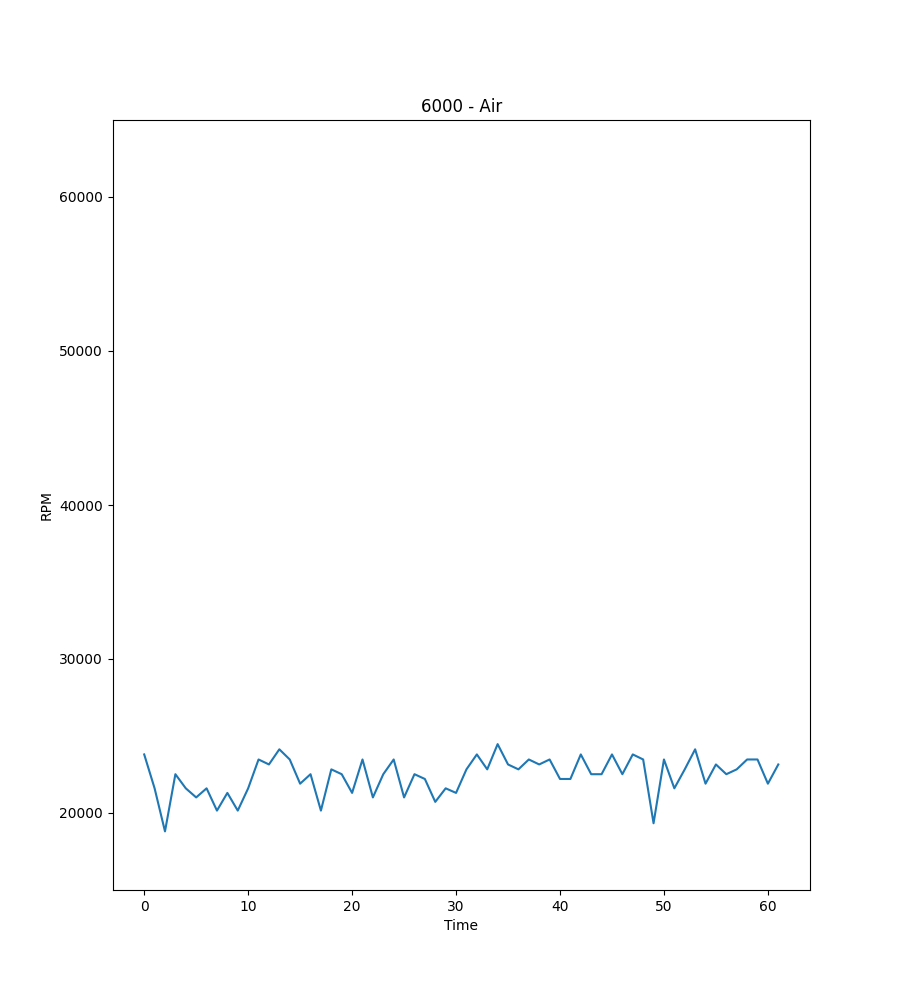
\includegraphics[width=0.5\linewidth]{Studienarbeit//images/cwt-6000-air-freqs-1.png}    
    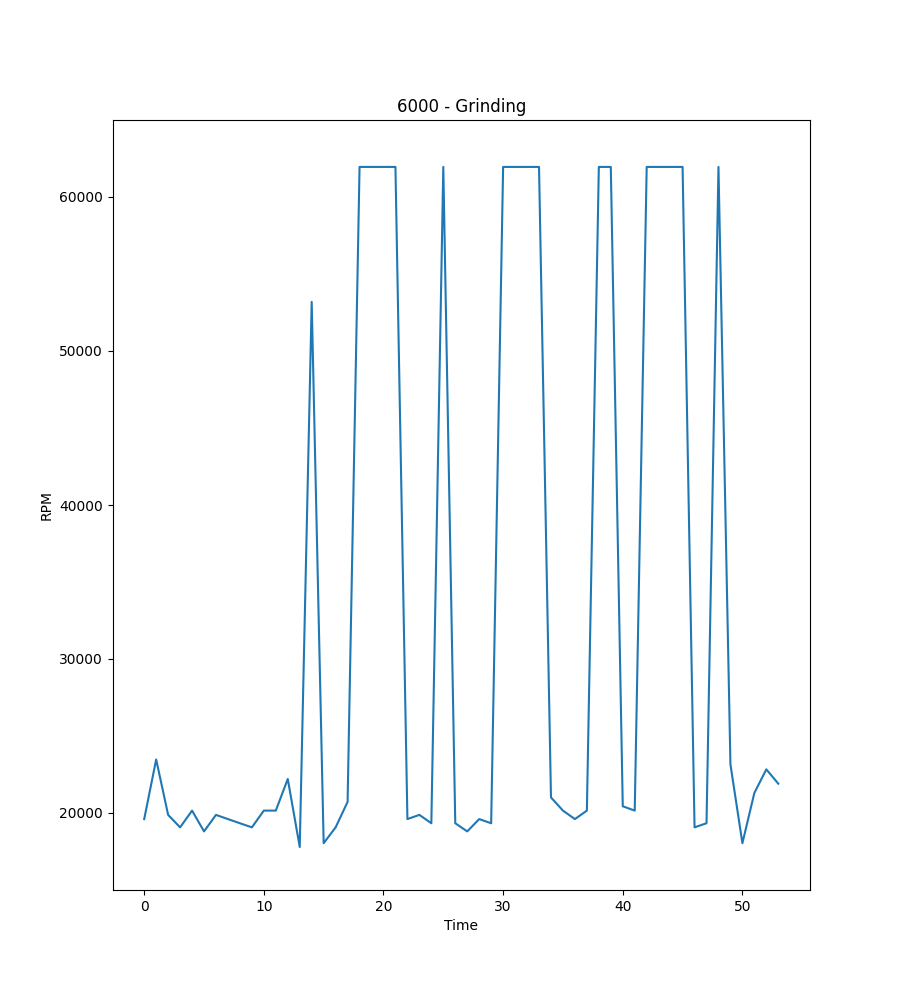
\includegraphics[width=0.5\linewidth]{Studienarbeit//images/cwt-6000-grinding-freqs-1.png}    
    \caption{Berechnung der am stärksten auftretenden Frequenz}
    \label{fig:cwt-iso-freqs}
\end{figure}

Hier zu erkennen ist deutlich, dass bei den Datensätzen, in welchem geschliffen wird tatsächlich viele Peaks im Bereich von 60000 RPM auftreten, welche der 10-fachen Drehzahl entsprechen, wobei erwähnt sein muss, dass es sich hierbei auch um Zufall handeln kann. Genauso wichtig zu erwähnen ist hierbei, dass die Quelle dieser Peaks unbekannt ist. So gibt es viele Faktoren, welche ein solches Rauschen verursachen können. Auch die Korrelation mit der Schleifleistung scheint hier zwar zu existieren, aber auch dabei kann es sich um Umstände handeln, die nur in genaue dieser exakten Umgebung des Roboters auftreten. Da diese Arbeit jedoch in erster Linie eine Machbarkeitsanalyse ist, die überprüft, ob überhaupt etwas aus den Daten heraus gelesen werden kann, wird an dieser Stelle mit diesen Daten weitergearbeitet und angenommen, dass die Frequenzen bei 60000 durch Schleifen erzeugt wird. Allen in allen wirken die Abbildungen recht ungenau und die gebildeten Platteua's bei 60000R RPM unnatürlich, weshalb sich im nächsten Schritt dafür entschieden wurde die Auflösung zu erhöhen. Dies wurde erreicht, indem das Zeitintervall, in welchem die stärkste Frequenz gesucht wird, verringert wird. Verschiedene dieser Zeitintervalle sind in der Abbildung \ref{fig:cwt-iso-freqs-genauigkeit} aufgezeigt. Grundlage für diese war immer das gleiche Audiosignal, um einen Vergleichswert zu schaffen.

\begin{figure}[H]
    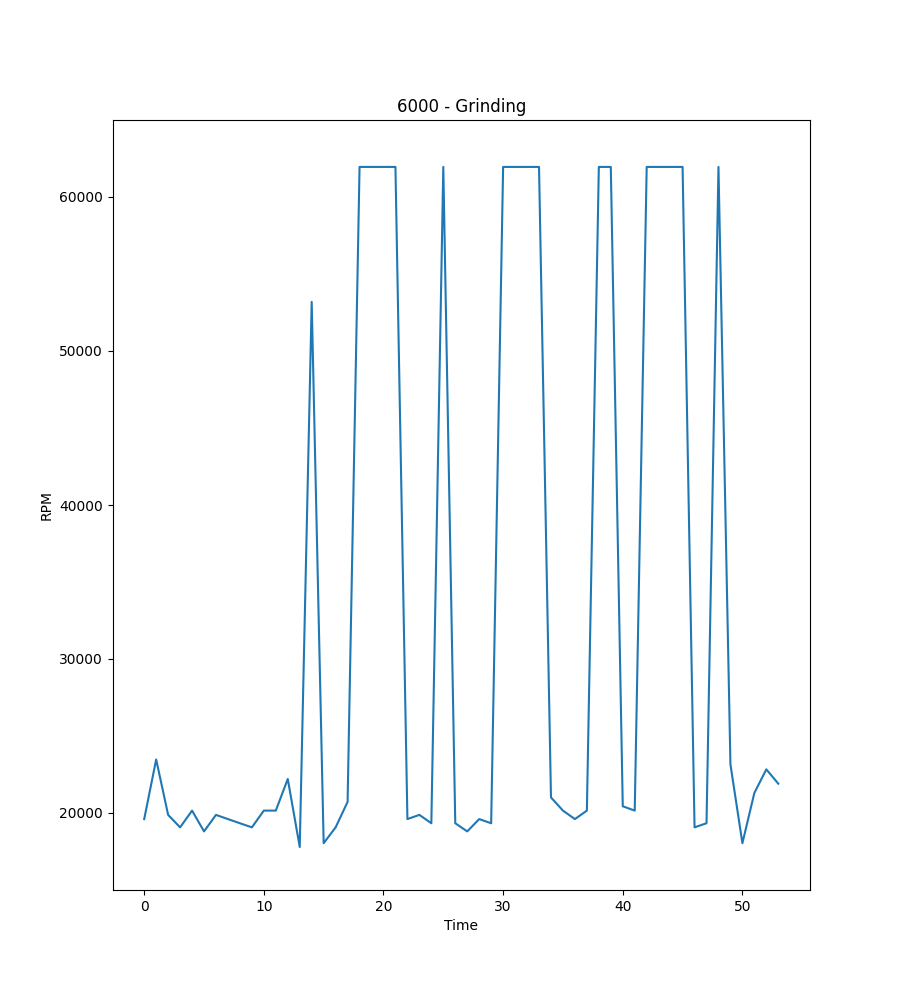
\includegraphics[width=0.5\linewidth]{Studienarbeit//images/cwt-6000-grinding-freqs-1.png} 
    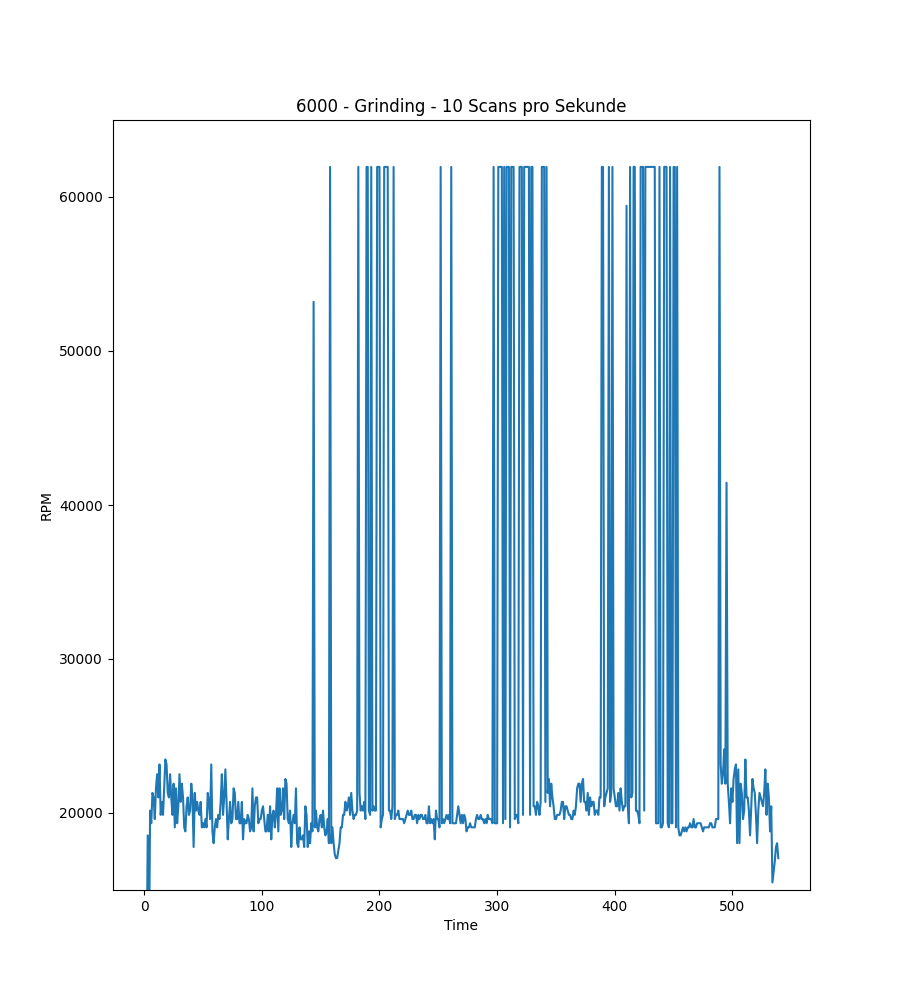
\includegraphics[width=0.5\linewidth]{Studienarbeit//images/cwt-6000-grinding-freqs-10.png}   
    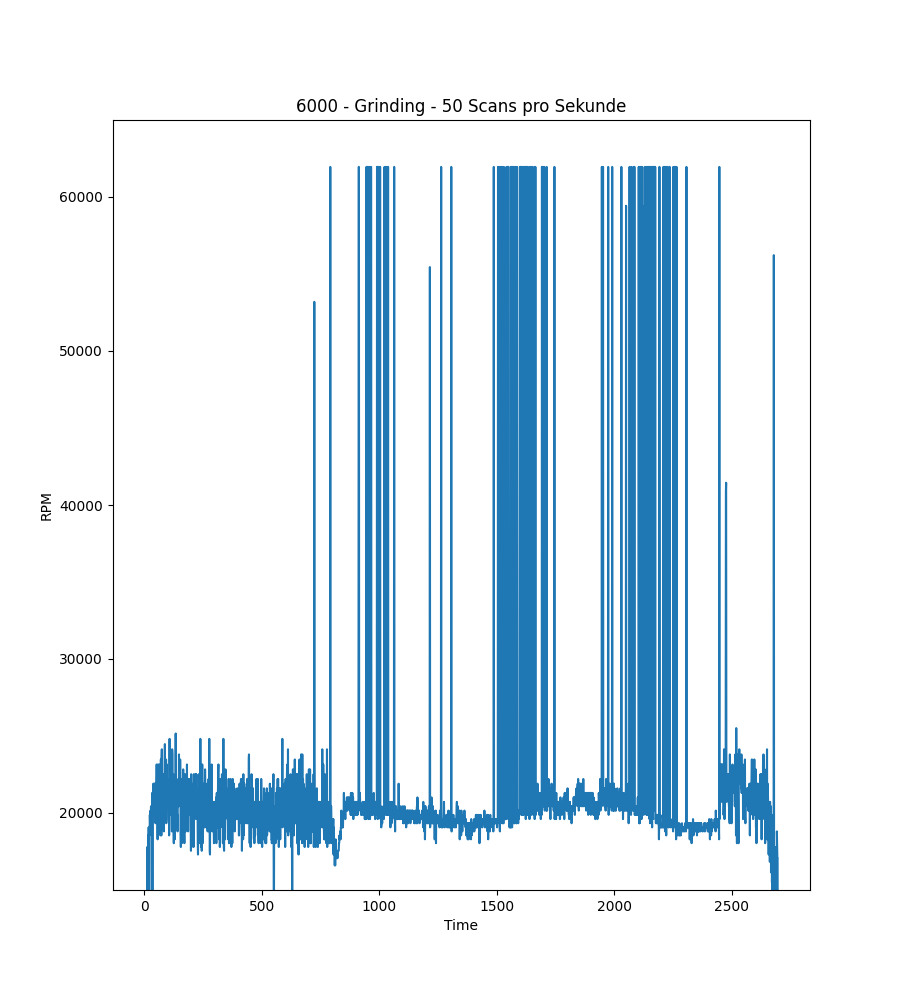
\includegraphics[width=0.5\linewidth]{Studienarbeit//images/cwt-6000-grinding-freqs-50.png}   
    \caption{Vergleich verschiedener zu untersuchende Zeitintervalle}
    \label{fig:cwt-iso-freqs-genauigkeit}
\end{figure}


Wie erwartet zeigt sich in höherer Auflösung, dass es sich bei den Plateaus, eigentlich nur um ganz viele Ganz kurze Peaks handelt. Dadurch wird klar, dass um die Schleifleistung zu bestimmen ein viel höherer Detaillierungsgrad notwendig ist, als zur Bestimmung der Drehzahl. Nun hat man   detaillierte Daten, welche Informationen über die Schleifleistung enthalten, diese müssen jetzt jedoch noch irgendwie richtig gedeutet werden. Eine Möglichkeit hierbei ist, sich den Mittelwert der Frequenzen innerhalb eines Zeitintervalls, z. B. einer Sekunde zu betrachten und mithilfe eines Grenzwertes festzulegen, ab welchem Mittelwert geschliffen wurde. Ein Mittelwert ist jedoch in der Hinsicht problematisch, dass die Frequenzen nicht bei 0 Anfangen und somit immer ein Bias existiert. Zwar könnte man auch in den Grenzwert mit einbeziehen, jedoch bietet die Stochastik genau dafür bereits eine Lösung an und zwar die Standardabweichung. Diese wird im nächsten Schritt berechnet, da diese selbst bei de gewählten Auflösung von 1/50s noch sehr kantig ist wird zusätzlich ein Mittelwert-Filter eingesetzt. Die Abbildung \ref{fig:cwt-std-mit-und-ohne-mittelwert-filter} zeigt nun diese Standardabweichung mit und ohne Mittelwert-Filter. 

\begin{figure}[H]
    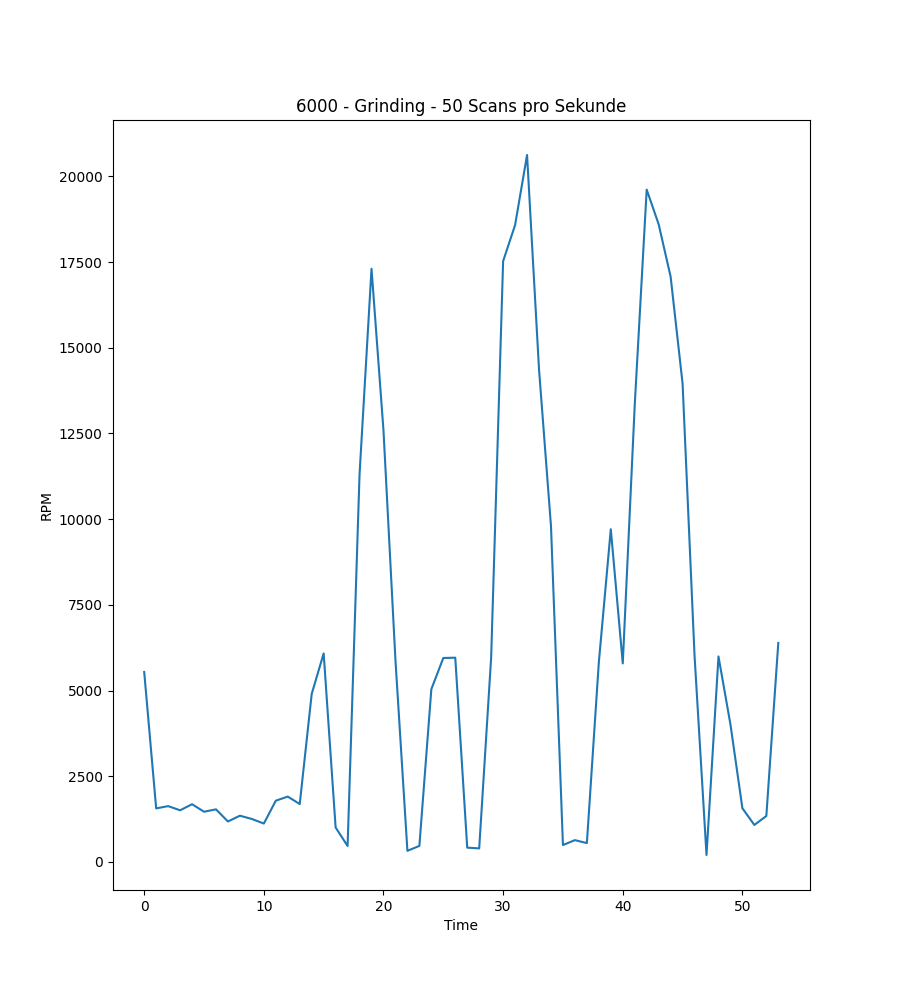
\includegraphics[width=0.5\linewidth]{Studienarbeit//images/cwt-6000-grinding-std.png} 
    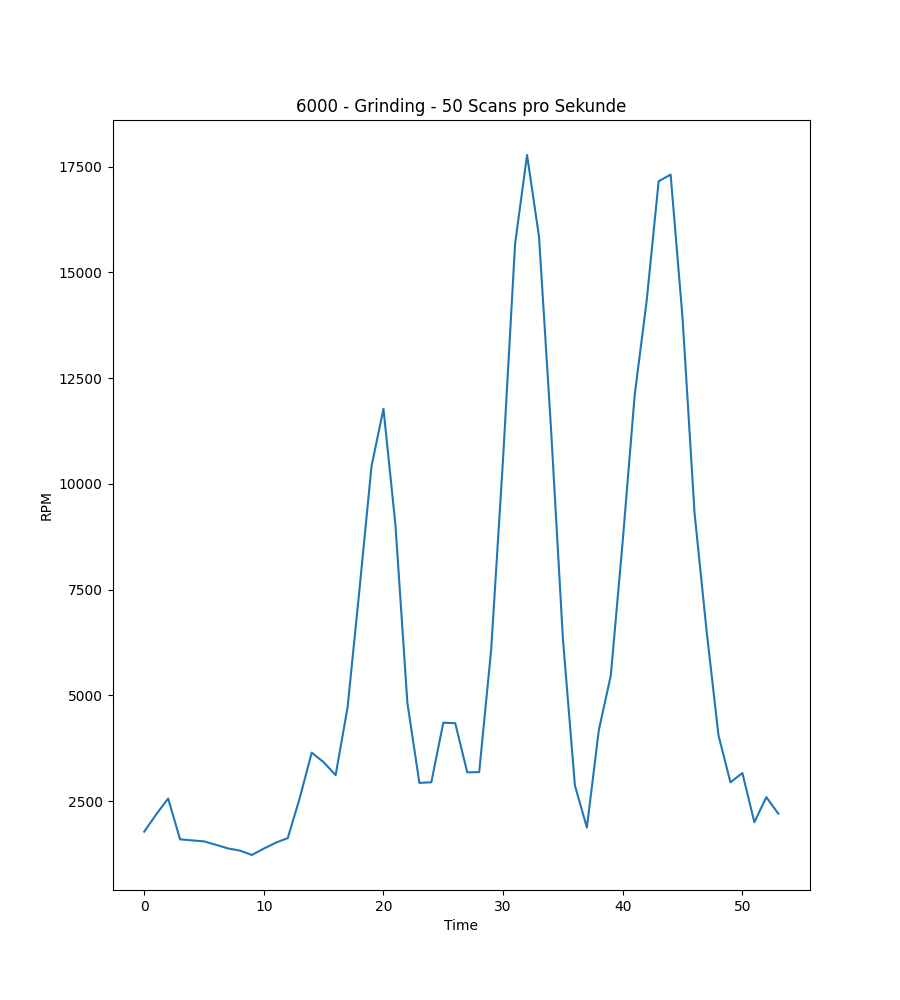
\includegraphics[width=0.5\linewidth]{Studienarbeit//images/cwt-6000-grinding-std-mw.png} 
    \caption{Standardabweichung mit und ohne Mittelwert-Filter}
    \label{fig:cwt-std-mit-und-ohne-mittelwert-filter}
\end{figure}

Da nun die Standardabweichung vorliegt muss ein Grenzwert festgelegt werden, aber welcher Standardabweichung ein Abschnitt als ,,Grinding'' eingeordnet hier. Durch die Auswertung mehrerer Datensätze fällt dieser Grenzwert auf 7500. Wichtig an dieser Stelle zu erwähnen ist, dass der Grenzwert vermutlich nur für eine Auswertung im Bereich von 6000 RPM gültig ist. Eine Berechnung dieses Grenzwertes ist an dieser Stelle leider nicht möglich, da es keine allgemeine Basis gibt, an welcher man sich orientieren kann. Zusätzlich kann sich der Grenzwert auch bei verschiedenen Materialien unterscheiden. Für den in Rahmen dieser Arbeit betrachte Schleifprozess ist dieser Grenzwert jedoch ausreichend und gibt sorgt für die grundlegende Erkenntnis darüber, dass eine akustische Vermessung eines robotischen Schleifprozesses funktionieren kann. Die Abbildung \ref{fig:cwt-schleif} zeigt nun das letztendliche Ergebnis mit einem von Grenzwert von 15000 auf verschiedene Audiosignale. Zur Veranschaulichung wurde ein Wert von 0 gewählt, wenn keine Schleifleistung erfolgt ist innerhalb der letzten Sekunde und ein Wert von 1 entspricht einer erbrachten Schleifleistung.

\begin{figure}[H]
    \centering
    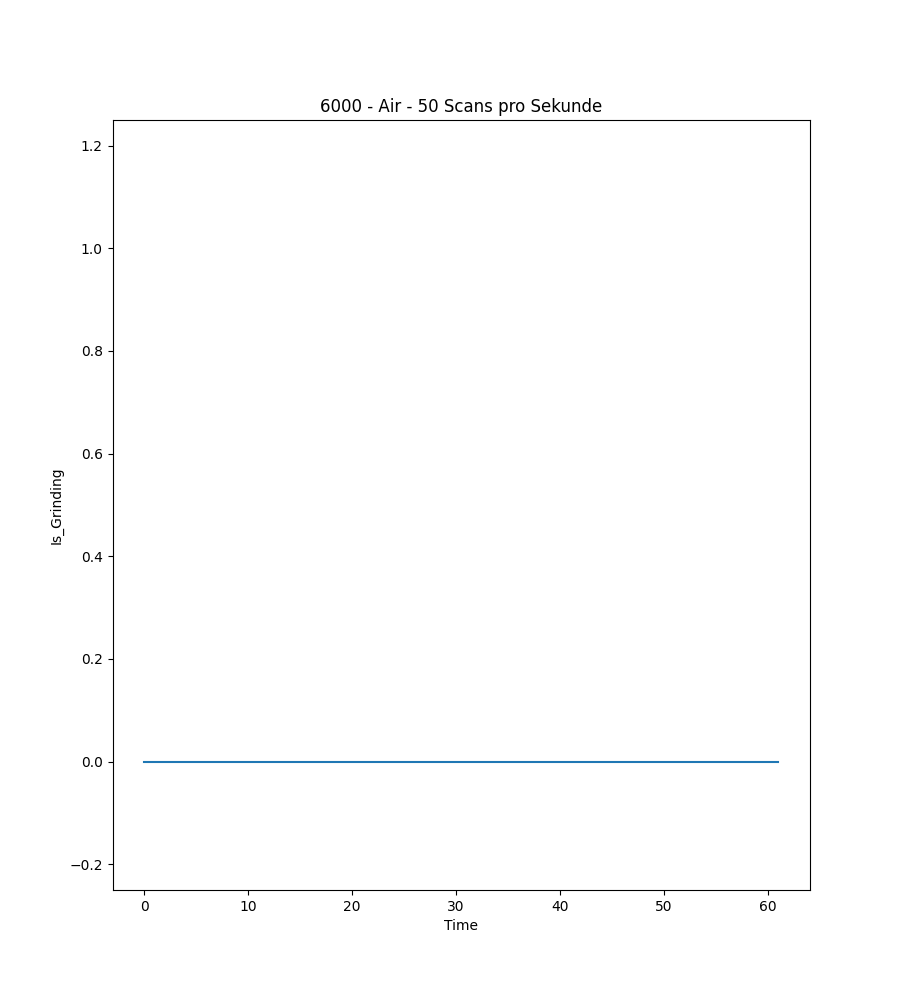
\includegraphics[width=0.44\linewidth]{Studienarbeit//images/cwt-6000-air-final-1.png} 
    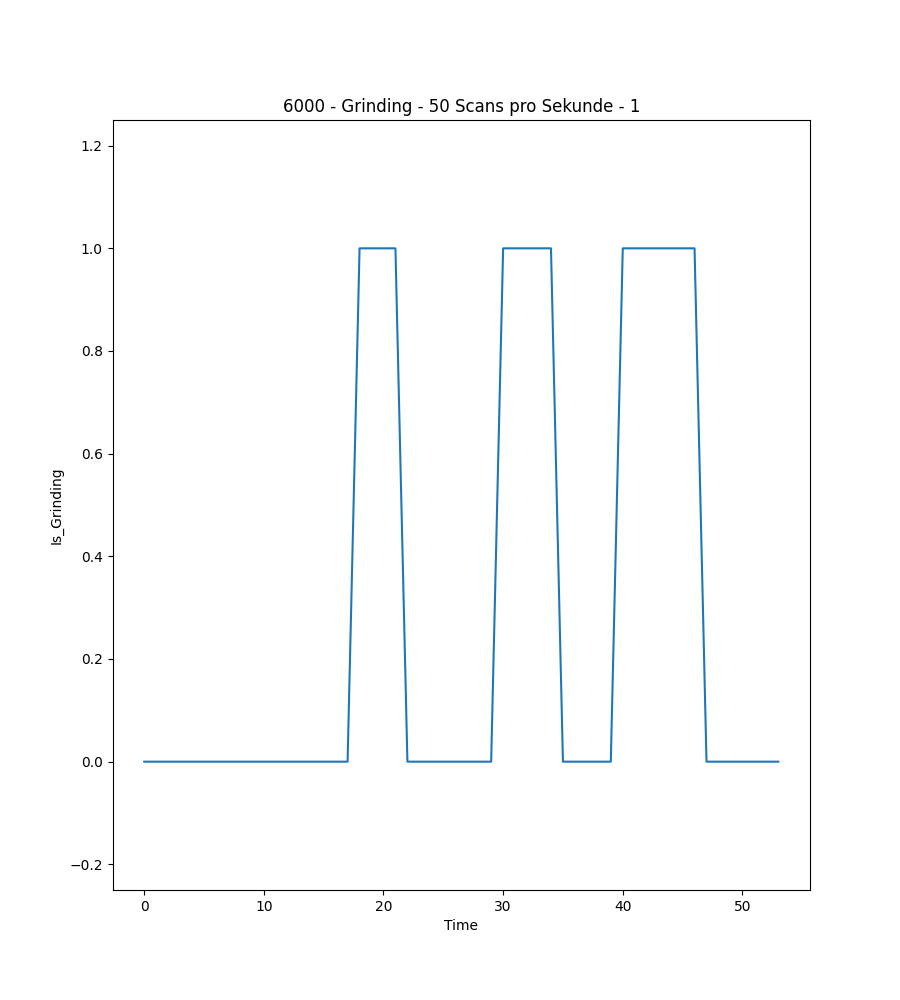
\includegraphics[width=0.44\linewidth]{Studienarbeit//images/cwt-6000-grinding-final-2.png}

    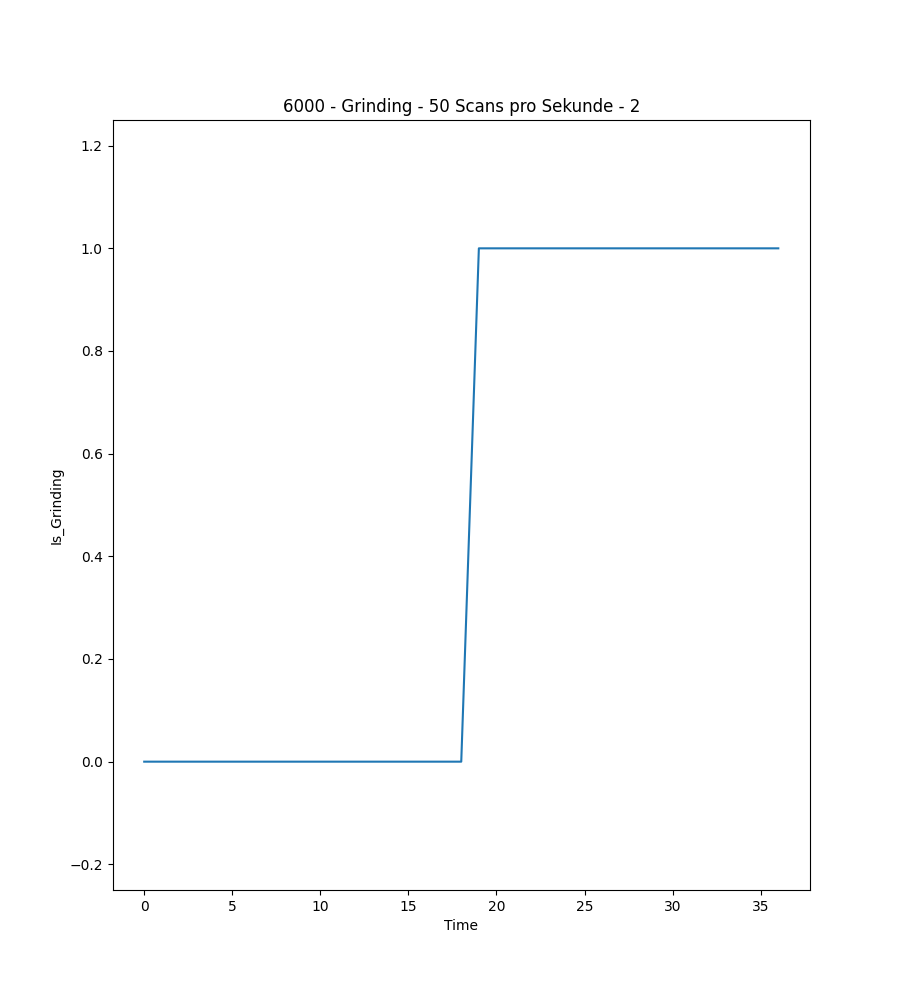
\includegraphics[width=0.44\linewidth]{Studienarbeit//images/cwt-6000-grinding-final-3.png} 
    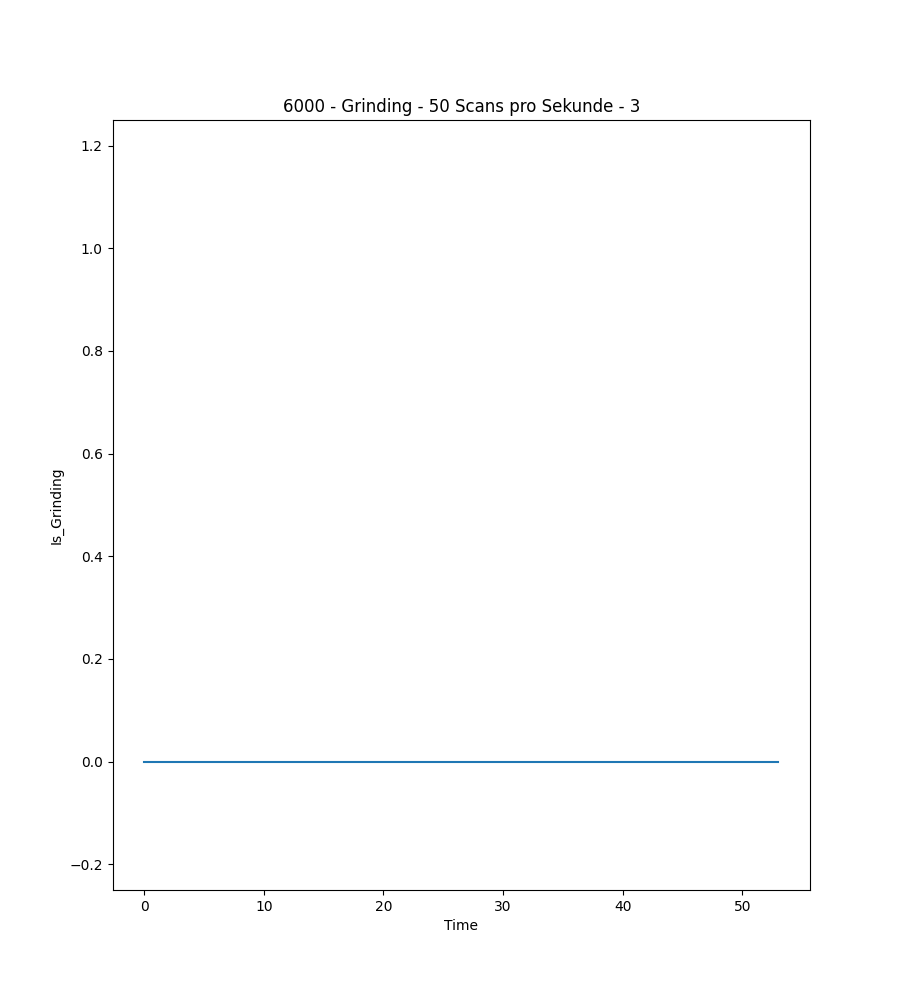
\includegraphics[width=0.44\linewidth]{Studienarbeit//images/cwt-6000-grinding-final-4.png} 
    \caption{Ergebnisse der Schleifleistung-Berechung}
    \label{fig:cwt-schleif}
\end{figure}

Die Ergebnisse zeigen deutlich, dass das Schleifgerät nicht zu jedem Zeitpunkt schleift. Auch bei den mit ,,Grinding'' markierten Audiosignalen kommt es so zu Zeitabschnitten, in welchen der Schleifer nicht schleift. Mithilfe einer solchen Darstellung kann nun analysiert werden, wie erfolgreich ein Schleifprozess war. Im folgenden Abschnitt werden nun die Ergebnisse dieser Durchführung nochmals zusammengefasst, zusätzlich werden Ideen für weitere Möglichkeiten erläutert, um diesen Prozess zu allgemeineren. Darin Anklang findet auch eine Klassifizierung mittels \ac{KI}, deren Umsetzbarkeit auch bereits im Kapitel \ref{Kapitel3} ausgiebig erläutert wurde.


\section{Ergebnis}
Im Letzten Kapitel wurden drei verschiedene Ansätze zur Audioanalyse getestet. Das Ziel war er herauszufinden, welche Informationen aus dem Audiosignal heraus gelesen werden können. Der erste Ansatz, welcher hier benutzt wurde war die \ac{FFT}, also eine Fourier-Transformationen. Diese ist bildete viele Jahre lang die Grundlage für jegliche Signalanalyse, so auch in diesem Anwendungsfall. Die Betrachtung der Audiosignale im Frequenzraum hat dazu geführt, dass sichtbar wurde, dass zum einen die Drehzahl des Schleifers zu erkennen ist, als auch ein Rauschen in den Audiosignalen, in denen geschliffen wurde. Nun ist jedoch auch der Fall, dass sichtbar wurde, dass bei einem SOLL von 4000RPM die stärkste Frequenz auf ein IST von 8000RPM hingedeutet hat. Dieses Problem ist vermutlich auf eine Eigenschwingung des Motors zurückzuführen, welche bei 4000RPM verstärkt wird. Diese Erkenntnis hat dann dazu beigetragen, dass sich in den Folgenden Ansätzen und bei der Analyse der Schleifleistung auf ein SOLL von 4000RPM beschränkt wurde. Letztendlich reichte die \ac{FFT} jedoch nicht aus um detaillierte Informationen sinnvoll auszulesen, weshalb sich dazu entschieden wurde der zeitlichen Komponente mehr Bedeutung zu geben. Hierfür wurde eine \ac{STFT} implementiert. Die Ergebnisse dieser \ac{STFT} bestätigten nochmals die Anomalie bei 4000RPM und bestätige auch, dass die Drehzahl bei SOLL 6000RPM abgelesen werden kann. Zudem wurden durch die zeitliche Komponente weitere Anomalien in den Ergebnissen sichtbar. Eine Anomalie lies auf ein Rauschen in den ersten 10 Sekunden jedes Audiosignals deuten, die andere Anomalie zeigt, dass allgemein viel mehr Rauschen in den Audiosignalen vorhanden ist, in welchen wahrscheinlich geschliffen wurde. Da jedoch auch diese Ergebnisse nicht sehr detailliert waren und zudem stark abhängig von den gewählten Parametern der STFT, kam schließlich eine\ac{CWT} zum Einsatz. Die Durchführung dieser verdeutlichte die davor aufgestellten Vermutungen und zeigte deutlich, dass die Berechnung der Drehzahl funktioniert. Zusätzlich offenbarte die\ac{CWT} auch, dass die Schleifleistung sich offenbar mit der dreifachen Frequenz korreliert, aus diesem Grund wurde die\ac{CWT} dann so verfeinert, dass dieser Frequenzbereich isoliert wurde. Die Auswertung zeigte dann jedoch, dass zwar auch die dreifache Drehzahl irgendwie mit der Schleifleistung zusammenhängt, viel auffälliger war hier jedoch ein Rauschen, welches sich im Bereich vom 5-10 fachen Drehzahlbereich befindet. Beim Auslesen der stärksten Frequenzen zeigte sich dann, dass im Falle einer erbrachten Schleifleistung zwischen der dreifachen-Drehzahl und der zehnfachen Drehzahl hin und her springen, während in Audiosignalen ohne Schleifleistung diese stärkste Frequenz konstant bei der dreifachen Drehzahl lag. Dies ermöglichte es dann anhand der Standardabweichung, der stärksten Drehzahl innerhalb eines Zeitintervalls, zu bestimmen, ob in diesem Zeitintervall geschliffen wurde oder nicht. Hierfür wurde ein fester Grenzwert festgesetzt. Soviel zu den erzielten Ergebnissen, nun folgt eine Bewertung dieser Ergebnisse. 

Auf den ersten Blick scheinen die Ergebnisse sehr gut zu sein, jedoch müssen hierbei einige Dinge beachtet werden. Erst einmal wurden alle Audiosignale in einer geschlossenen Atmosphäre aufgenommen, wobei immer das gleiche Material geschliffen wurde. Zusätzlich ist es möglich, dass gewisse Anomalien gar nicht durch das Schleifen selbst, sondern durch beispielsweise die Befestigung des Materials entstand. So ist es möglich, dass diese gefundene Anomalie bei der 10-fachen Drehzahl also nicht auf das Schleifen zurückzuführen ist und nur in genau dieser Prototypischen Umgebung existiert, in der geschliffen wurde. Dies führt zeitgleich auch dazu, dass dieser festgelegte Grenzwert möglicherweise nur in dieser Umgebung gute Ergebnisse liefert. Auch wichtig anzumerken ist, dass es nur möglich war diese Erkenntnisse bei Audiosignalen zu treffen, welche im Bereich von 6000 RPM aufgenommen wurde. Bei 4000 RPM trat Rauschen auf, welches es nicht ermöglichte automatische Analysen zu machen. Insgesamt lässt sich hier also festhalten, dass die erzielten Ergebnisse mit Vorsicht zu betrachten sind und die Methoden zur Analyse der RPM und der Schleifleistung nur in diesem prototypischen Umfeld gute Ergebnisse erzielen kann.

Insgesamt zeigen aber genau diese Ergebnisse, dass es möglich ist Methoden zu entwickeln, welche eine prädiktive Wartung ermöglichen. Aus diesem Grund haben wir uns auch dafür entschieden in Kapitel \ref{Kapitel3} mögliche State of the Art Lösungen zum Thema KI zu betrachten. Die verschiedenen Ergebnisse zeigen deutlich, dass Muster in den Daten zu erkennen sind. Diese Muster gilt es nur auszulesen. Dies ist mit ,,einfachen'' Algorithmen nicht gelungen, doch der Einsatz von KI scheint hier erfolgversprechend zu sein, da wie bereits erwähnt ähnliche Klassifizierungen und Analysen in diesem Bereich bereits mit Erfolg in diesem Bereich durchgeführt wurden. Klar stellt sich nun die Frage, wieso diese Arbeit die Analyse mit KI nicht in Betracht gezogen hat. Der Grund dafür liegt darin, dass die Datengrundlage viel zu gering ist, um eine KI von neu auf zu trainieren. So wäre es notwendig gewesen mehrere Tausende Daten manuell aufzunehmen und zu Labeln, wobei nicht mal sichergestellt ist, dass die Label richtig sind. Aus diesem Grund lag die Entscheidung nahe, dass es erst mal wichtig ist grundsätzlich die Daten zu analysieren, um aufzuklären, ob überhaupt Muster in den Daten zu erkennen sind, die dann von einer KI analysiert werden können. Zusätzlich zeigt diese Arbeit auch Möglichkeiten zur Vorverarbeitung von Daten und ermöglicht es zugleich, dass nicht alle Daten manuell gelabelt werden müssen, sondern der aufgezeigte Algorithmus dieses Labeln übernehmen kann. Manuell müssen diese Labels dann nur noch stichprobenartig überprüft werden. Insgesamt zeigt diese Arbeit also auf, dass sehr wohl die grundsätzliche Möglichkeit besteht, Eigenschaften über den Schleifprozess aus den Audiosignalen aus.


%%%%%%%%%%%%%%%%%%%%%%%%%%%%%%%%%%%%%%%%%%%%%%%%%%%%%%%%%%%%%%%%%%%%%%%%%%%%%%%
\endinput
%%%%%%%%%%%%%%%%%%%%%%%%%%%%%%%%%%%%%%%%%%%%%%%%%%%%%%%%%%%%%%%%%%%%%%%%%%%%%%%
